\documentclass{beamer}
\usetheme{Frankfurt}
\usepackage[utf8]{inputenc}
\usepackage{charter}
\usepackage{tikz}
\usepackage{graphicx}
\usepackage{amsmath}
\usepackage{amssymb}
\usepackage{listings}
\usepackage{animate}
\usepackage{mathtools}
\mathtoolsset{showonlyrefs}
\usepackage{caption}
\captionsetup[figure]{labelformat=empty}
\usepackage{tikz}
\usepackage{tikz-cd}
\usetikzlibrary{arrows,chains,matrix,positioning,scopes,cd}
\usepackage{tikzit}
\documentclass{beamer}
\usetheme{Frankfurt}
\usepackage[utf8]{inputenc}
\usepackage{charter}
\usepackage{tikz}
\usepackage{graphicx}
\usepackage{amsmath}
\usepackage{amssymb}
\usepackage{listings}
\usepackage{animate}
\usepackage{mathtools}
\mathtoolsset{showonlyrefs}
\usepackage{caption}
\captionsetup[figure]{labelformat=empty}
\usepackage{tikz}
\usepackage{tikz-cd}
\usetikzlibrary{arrows,chains,matrix,positioning,scopes,cd}
\usepackage{tikzit}
\documentclass{beamer}
\usetheme{Frankfurt}
\usepackage[utf8]{inputenc}
\usepackage{charter}
\usepackage{tikz}
\usepackage{graphicx}
\usepackage{amsmath}
\usepackage{amssymb}
\usepackage{listings}
\usepackage{animate}
\usepackage{mathtools}
\mathtoolsset{showonlyrefs}
\usepackage{caption}
\captionsetup[figure]{labelformat=empty}
\usepackage{tikz}
\usepackage{tikz-cd}
\usetikzlibrary{arrows,chains,matrix,positioning,scopes,cd}
\usepackage{tikzit}
\documentclass{beamer}
\usetheme{Frankfurt}
\usepackage[utf8]{inputenc}
\usepackage{charter}
\usepackage{tikz}
\usepackage{graphicx}
\usepackage{amsmath}
\usepackage{amssymb}
\usepackage{listings}
\usepackage{animate}
\usepackage{mathtools}
\mathtoolsset{showonlyrefs}
\usepackage{caption}
\captionsetup[figure]{labelformat=empty}
\usepackage{tikz}
\usepackage{tikz-cd}
\usetikzlibrary{arrows,chains,matrix,positioning,scopes,cd}
\usepackage{tikzit}
\input{main.tikzstyles}
\beamertemplatenavigationsymbolsempty
\let\vec\mathbf
\newcommand{\norm}[1]{\left\lVert#1\right\rVert}
\newcommand{\abs}[1]{\left|#1\right|}
\DeclareMathOperator{\Forall}{\forall}


%% Title slide formatting %%

\pgfdeclareimage[width=\paperwidth]{titlebackground}{Images/title-slide-background.png}
\setbeamerfont{subtitle}{size=\tiny}
\setbeamertemplate{endpage}{
	\begin{picture}(0,0)
		\scalebox{1.01}{
		\put(-28.5,-163){%
			\pgfuseimage{titlebackground}
		}
		}
		\put(0,-115){%
			\begin{minipage}[b][4.5cm][t]{0.5\textwidth}
				\color{white}
				\usebeamerfont{title}
				{\textbf{Thank Your} \\ \textbf{For You Attention !}}
			\end{minipage}
		}
	\end{picture}
}
\setbeamertemplate{title page}{
	\begin{picture}(0,0)
		\scalebox{1.01}{
			\put(-28.5,-163){%
				\pgfuseimage{titlebackground}
			}
		}
		\put(0,-75){%
			\begin{minipage}[b][4.5cm][t]{0.7\textwidth}
				\color{white}
				\usebeamerfont{title}
				{\inserttitle\\[0.9cm]}
				\usebeamerfont{subtitle}
				{\insertauthor\par}
				{\insertinstitute\\[0.3cm]}
				{\insertdate}
			\end{minipage}
		}
	\end{picture}
}


%% General slide formatting %%

\definecolor{oxfordblue}{RGB}{4,30,66}

\pgfdeclareimage[width=0.9cm]{oxfordlogo}{Images/oxford-logo.png}
\pgfdeclareimage[width=1cm]{mathslogo}{Images/mathematics-logo.png}
\pgfdeclareimage[width=0.9cm]{pizzalogo}{Images/pizza-logo.png}

\setbeamertemplate{headline}
{%
	\begin{picture}(0,0)
		\put(314,-50){%
			\pgfuseimage{oxfordlogo}
		}
		\put(20,-55){%
			\rule{320pt}{0.4pt}
		}
	\end{picture}
}

\setbeamertemplate{frametitle}
{%
	\begin{picture}(0,0)
		\put(-8,-20){%
			\normalsize\textbf{\color{oxfordblue}\insertframetitle}
		}
		\put(-7,-25){%
			\small\color{oxfordblue}\insertframesubtitle
		}
	\end{picture}
}

\setbeamertemplate{footline}
{%
	\begin{picture}(0,0)
		\put(20,30){%
			\rule{320pt}{0.4pt}
		}
		\put(20,14){%
			\pgfuseimage{mathslogo}
		}
		\put(100,14){%
			\color{oxfordblue}\insertshortdate
		}
		\put(160,14){%
			\color{oxfordblue}\insertshorttitle
		}
		\put(337,14){%
			\color{oxfordblue}\insertframenumber
		}
	\end{picture}%
}
\setbeamercolor{block title}{bg=oxfordblue!30,fg=black}

\definecolor{codegreen}{rgb}{0,0.6,0}
\definecolor{codegray}{rgb}{0.5,0.5,0.5}
\definecolor{codepurple}{rgb}{0.58,0,0.82}
\definecolor{backcolour}{rgb}{0.95,0.95,0.92}

\lstdefinestyle{mystyle}{
	%backgroundcolor=\color{backcolour},   
	commentstyle=\color{codegray},
	keywordstyle=\color{oxfordblue},
	numberstyle=\tiny\color{codegray},
	stringstyle=\color{codegreen},
	basicstyle=\ttfamily\footnotesize,
	breakatwhitespace=false,         
	breaklines=true,                 
	captionpos=b,                    
	keepspaces=true,                 
	numbers=left,                    
	numbersep=5pt,                  
	showspaces=false,                
	showstringspaces=false,
	showtabs=false,                  
	tabsize=2
}

\lstset{style=mystyle}

%% Information (author, title, etc.) %%

\title[Divergence-free discretisations of the Stokes eigenvalue problem]{Divergence-free discretisations of the Stokes eigenvalue problem} % short title for footer
\author%
{%
	\sc{Fleurianne Bertrand}\;*, \sc{Daniele Boffi}$\;\dagger$, \underline{\sc{U. Zerbinati}}$\;\ddagger$\\
}
\institute%
{%
	* \textit{Chemnitz University of Technology}
	\\
	$\;\dagger\;$\textit{King Abdullah University of Science and Technology}
	\\
	$\;\ddagger\;$\textit{University of Oxford}
}

\date[EFEF 2023]{European Finite Element Fair, 12th of May 2023\\ \\
\texttt{https://github.com/UZerbinati/EFEF2023}} % short date for footer



%% Content of slides %%

\begin{document}
	\begin{frame}[plain]
		\titlepage
	\end{frame}
	\begin{frame}
		\frametitle{Stokes eigenvalue problem}
		Find $(\vec{u},p)\!\in\!C^2_{0}(\Omega)\!\times\!\big[C^1(\Omega)\backslash \mathbb{R}\big]$ such that: 
		\begin{align}
			\nu\Delta \vec{u} - \nabla p &= \lambda \vec{u}\nonumber\\
			\nabla\cdot \vec{u} &= 0\nonumber
		\end{align}
		\begin{itemize}
			\item<2->[\color{oxfordblue}$\blacktriangleright$] The Stokes flow is characterized by advective inertial forces extremely small compared with viscous forces. 
			\item<3->[\color{oxfordblue}$\blacktriangleright$] Stokes flow can be used to model lubrication and viscous colloidal suspensions.
		\end{itemize}
	\end{frame}
	\begin{frame}
		\frametitle{The applications}
		\begin{itemize}
			\item [\color{oxfordblue}$\blacktriangleright$] The eigenfunctions of the Stokes eigenproblem span the space where solutions of the full Navier-Stokes equations are sought. 
		\end{itemize}
		$\newline$
		\begin{minipage}{0.45\textwidth}
			\begin{itemize}
				\item<2->[\color{oxfordblue}$\blacktriangleright$] The eigenvalues of the Stokes eigenproblem play a crucial role in computing a critical value for the Raynolds number, above which we will predict instabilities in Coutte flow.
			\end{itemize}
		\end{minipage}
		\qquad
		\begin{minipage}{0.45\textwidth}
			\visible<2->{
			\begin{figure}
				\centering
				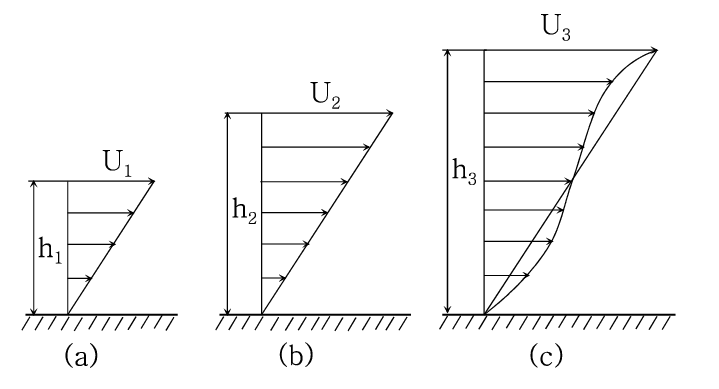
\includegraphics[scale=0.2]{Figures/Couette}
			\end{figure}
			}
		\end{minipage}
	\end{frame}
	\begin{frame}
		\frametitle{Our contribution}
		\begin{itemize}
			\item<1->[\color{oxfordblue}$\blacktriangleright$] We analyze divergence-free discretisations for the Stokes eigenvalue problem, and prove their well-posedness \textbf{\color{oxfordblue}independently} from the \textbf{\color{oxfordblue}characterization} of \textbf{\color{oxfordblue}the range} of the \textbf{\color{oxfordblue}discrete divergence operator}. 
			\item<2>[\color{oxfordblue}$\blacktriangleright$] We develop a systematic approach to \textbf{\color{oxfordblue}best approximation estimates} for functions living in the \textbf{\color{oxfordblue}kernel} of the \textbf{\color{oxfordblue}discrete divergence operator}, using \textbf{\color{oxfordblue}finite element exterior calculus}.
		\end{itemize}
	\end{frame}
	\begin{frame}
		\frametitle{Weak Stokes eigenvalue problem}
		$\newline$ 
		Find $(\vec{u},p)\!\in\!H^1_{0}(\Omega)\!\times\!\mathcal{L}^2_0(\Omega)$ such that $\Forall (\vec{v},q)\!\in\!H^1_0(\Omega)\!\times\!\mathcal{L}^2_0(\Omega)$,
		\begin{align*}
				\nu(\nabla \vec{u},\nabla \vec{v})_{\mathcal{L}^2(\Omega)}-(\nabla\cdot \vec{v},p)_{\mathcal{L}^2(\Omega)}&=\lambda_n\; (\vec{u},\vec{v})_{\mathcal{L}^2(\Omega)},\\
				(\nabla \cdot \vec{u}, q)_{\mathcal{L}^2(\Omega)} &= 0, 
		\end{align*}
		with $\lambda_n\in \mathbb{C}$, and $\nu\in \mathbb{R}_{> 0}$ is the fluid viscosity. 
		$\newline$
		\begin{itemize}
			\item<2->[\color{oxfordblue}$\blacktriangleright$] Are the eigenvalue of this problem real?
			\item<3->[\color{oxfordblue}$\blacktriangleright$] Do the eigenvalue of this problem diverge?
		\end{itemize}
	\end{frame}
	\begin{frame}
		\frametitle{Weak Stokes eigenvalue problem -- Laplace form}
		$\newline$ 
		$\newline$ 
		We introduce the space $H^1_{0,0}(\Omega)=\Big\{\vec{v}\in H^1_0(\Omega) \;:\; \nabla\cdot \vec{u} = 0 \Big\}$.
		\\
		$\newline$
		Find $\vec{u}\!\in\!H^1_{0,0}(\Omega)$ such that $\Forall \vec{v}\!\in\!H^1_{0,0}(\Omega)$,
		\begin{equation*}
				\nu(\nabla \vec{u},\nabla \vec{v})_{\mathcal{L}^2(\Omega)}=\lambda_n \;(\vec{u},\vec{v})_{\mathcal{L}^2(\Omega)},\label{eq:}
		\end{equation*}
		with $\lambda_n\in \mathbb{C}$, and $\nu\in \mathbb{R}_{> 0}$ is the fluid viscosity. 
		\vspace{0.2cm}
		\begin{itemize}
			\item<2->[\color{oxfordblue}$\blacktriangleright$] The eigenvalue problem is self-adjoint therefore $\lambda_n\in \mathbb{R}$.
			\item<3->[\color{oxfordblue}$\blacktriangleright$] $H^1_{0,0}(\Omega)$ is compactly embedded in $\mathcal{L}^2(\Omega)$ and therefore operator corresponding to the eigenvalue problem is compact, implying $\lambda_n \to \infty$ as $n\to\infty$.
		\end{itemize}
	\end{frame}
	\begin{frame}
		\frametitle{Discrete weak Stokes eigenvalue problem}
		$\newline$
		$\newline$
		$\newline$
		Find $(\vec{u}^h,p^h)\!\in\!V_h\!\times\!Q_h$ such that $\Forall\,(\vec{v}^h,q^h)\in V_h\times Q_h$,
		\begin{align*}
				\nu(\nabla \vec{u}^h,\nabla \vec{v}^h)_{\mathcal{L}^2(\Omega)}-(\nabla\cdot \vec{v}^h,p^h)_{\mathcal{L}^2(\Omega)}&=\lambda_n\; (\vec{u}^h,\vec{v}^h)_{\mathcal{L}^2(\Omega)},\\
				(\nabla \cdot \vec{u}^h, q^h)_{\mathcal{L}^2(\Omega)}&= 0, 
		\end{align*}
		with $\lambda_n^h\in \mathbb{C}$, $\nu\in \mathbb{R}_{> 0}$ is the fluid viscosity, and 
		\begin{equation*}
			\boxed{
				V_h\!\times\! Q_h \!\subset \!H^1_0(\Omega)\!\times\!\mathcal{L}^2_0(\Omega).
			}
		\end{equation*}
		\vspace{-0.5cm}
		\visible<2->{
			\begin{center}
				\color{oxfordblue} \textbf{Under what hypotheses on $V_h$ and $Q_h$ is  this eigenvalue problem well-posed ?}
			\end{center}
		}
	\end{frame}
	\begin{frame}{Babu\v{s}ka--Banach--Brezzi condition}
		\begin{columns}[T] 
			\begin{column}{0.65\textwidth} 
			
			\vspace{0.2cm} 
			\begin{block}{\textbf{\color{oxfordblue} Inf-Sup}}
				The \textbf{\color{oxfordblue}necessary} and \textbf{\color{oxfordblue}sufficient} condition for the well-posedness of the \textbf{\color{oxfordblue}source} problem is given by the \textbf{\color{oxfordblue}inf-sup} condition, i.e.
				\begin{equation}
					\underset{p_h \in Q_h}{\inf}\;\;\underset{\vec{v}_h\in V_h}{\sup} \frac{(\nabla\cdot v_h,p_h)_{\mathcal{L}^2(\Omega)}}{\norm{\vec{v}_h}_{H^1(\Omega)}\norm{p_h}_{\mathcal{L}^2(\Omega)}}\geq \beta,\nonumber 
				\end{equation}
				where $\beta$ ideally is independent of $h$.
			\end{block}
			\end{column} 
			
			\begin{column}{0.35\textwidth} 
				\vspace{1cm}
				\begin{figure} 
					\centering 
					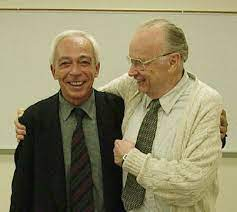
\includegraphics[width=1\textwidth]{Figures/BBB.jpeg} 
					\caption*{\tiny{F. Brezzi and I. Babu\v{s}ka}} 
				\end{figure} 
			\end{column} 
		\end{columns} 
	\end{frame}
	\begin{frame}{Boffi-Brezzi-Gastaldi observation}
		\begin{columns}[T] 
			\begin{column}{0.65\textwidth} 
			
			\vspace{0.2cm} 
			\begin{alertblock}{\textbf{Necessary and sufficient conditions}}
				When it comes to the eigenvalue problem, the inf-sup condition is \textbf{neither necessary nor sufficient}.
			\end{alertblock}
			\visible<2->{
				\begin{block}{\textbf{\color{oxfordblue}Q1-P0 Example}}
					Boffi, Brezzi and Gastaldi, showed that the \textbf{\color{oxfordblue} Q1-P0} finite element pair will lead to a converging eigenvalue problem, even if for this choice of element pair $\beta(h)\searrow 0$ as $h\to 0$.
				\end{block}
			}
			\end{column} 
			
			\begin{column}{0.35\textwidth} 
				\begin{figure} 
					\centering 
					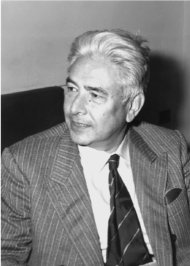
\includegraphics[width=0.8\textwidth]{Figures/DeGiorgi.jpg} 
					\caption*{\tiny{Enio De Giorgi, 1928--1996}} 
				\end{figure} 
			\end{column} 
		\end{columns} 
	\end{frame}
	\begin{frame}
		\frametitle{Boffi--Brezzi--Gastaldi conditions for Stokes}
		$\newline$
		\begin{itemize}
			\item<1->[\color{oxfordblue}$\blacktriangleright$] We say that $Q_h$ verifies the \textbf{\color{oxfordblue}weak approximability condition} if there exists $\gamma_1(h)$, such that for every $q \in \mathcal{L}^2_0(\Omega)$
				\begin{equation*}
					\underset{\vec{v}^h \in \mathbb{K}_h}{\sup} \frac{(\nabla\cdot\vec{v}^h,q)}{\norm{\vec{v}_h}_{H^1(\Omega)}} \leq \omega_1(h) \norm{q}_{\mathcal{L}^2(\Omega)} \; and \; \underset{h\to 0}{\lim}\,\gamma_1(h)=0.
				\end{equation*}
			\item<2->[\color{oxfordblue}$\blacktriangleright$] We say $V_h$ verifies the \textbf{\color{oxfordblue}strong approximability condition} if there exists $\gamma_2(h)$, such that for every $\vec{v} \in H^1_{0,0}(\Omega)\cap H^2(\Omega)$ 
				\begin{equation*}
					\underset{\vec{v}^h \in \mathbb{K}_h}{\inf} \norm{\vec{v}-\vec{v}^h}_{H^1(\Omega)} \leq \gamma_2(h)\norm{\vec{v}}_{H^2(\Omega)}\; and \; \underset{h\to 0}{\lim}\,\gamma_2(h)=0.
				\end{equation*}
		\end{itemize}
	\end{frame}
	\begin{frame}
		\frametitle{The divergence-free constraint}
		$\newline$
		$\newline$
		\begin{equation*}
			\boxed{
				b(\vec{v}^h,q^h)=(\nabla \cdot \vec{v}^h, q^h)_{\mathcal{L}^2(\Omega)}=0	
			}
		\end{equation*}
		$\newline$
		\visible<2->{
			Find $\vec{u}_h\!\in\!\mathbb{K}_{h}$ such that $\Forall \vec{v}_h\!\in\!\mathbb{K}_{h}$,
			\begin{equation*}
					\nu(\nabla \vec{u}^h,\nabla \vec{v}^h)_{\mathcal{L}^2(\Omega)}=\lambda_n^h \;(\vec{u}^h,\vec{v}^h)_{\mathcal{L}^2(\Omega)},
			\end{equation*}
			with $\lambda_n\in \mathbb{C}$, $\nu\in \mathbb{R}_{> 0}$ is the fluid viscosity and 
			\begin{equation*}
				\mathbb{K}_h=\Big\{\vec{v}^h\in V_h \;:\; b(\vec{v}^h,q^h) = 0, \Forall q^h\!\in\!Q_h\Big\}.
			\end{equation*}
		}
		\vspace{-0.3cm}
		\visible<3->{
			\begin{equation*}
				\boxed{\mathbb{K}_h\not\subset H^1_{0,0}(\Omega)}
			\end{equation*}
		}
	\end{frame}
	\begin{frame}
		\frametitle{Divergence-free discretisations}
		$\newline$
		\begin{equation*}
			\boxed{\nabla\cdot V_h\subset Q_h}
		\end{equation*}
		$\newline$
		\visible<2->{
			Under this hypothesis, we have the following result, i.e.
			\begin{equation*}
				b(\vec{v}^h,q^h)=(\nabla \cdot \vec{v}^h, q^h)_{\mathcal{L}^2(\Omega)}=0	\Leftrightarrow \nabla\cdot \vec{v}^h=0,
			\end{equation*}
			which implies the functions are point-wise \textbf{\color{oxfordblue}divergence-free}.
		}
		\visible<3->{
		\begin{equation*}
			\boxed{\mathbb{K}_h\subset H^1_{0,0}(\Omega)}
		\end{equation*}
		}
	\end{frame}
	\begin{frame}
		\frametitle{Divergence discretisations eigenvalue problem}
		$\newline$
		Find $\vec{u}_h\!\in\!\mathbb{K}_{h}$ such that $\Forall \vec{v}_h\!\in\mathbb{K}_{h}$,
		\begin{equation*}
				\nu(\nabla \vec{u}^h,\nabla \vec{v}^h)_{\mathcal{L}^2(\Omega)}=\lambda_n^h \;(\vec{u}^h,\vec{v}^h)_{\mathcal{L}^2(\Omega)},\label{eq:}
		\end{equation*}
		with $\nabla\cdot V_h\subset Q_h$, $\lambda_n\in \mathbb{C}$, $\nu\in \mathbb{R}_{> 0}$ is the fluid viscosity. 
		$\newline$
		\visible<2->{
			\begin{center}
				\color{oxfordblue} \textbf{This problem is well-posed and we can analyse it using Babu\v{s}ka-Osborn theory.}
			\end{center}
		}
	\end{frame}
	\begin{frame}
		\frametitle{Babu\v{s}ka--Osborn theory}
		\vspace{0.5cm}
		\begin{theorem}
			For each $n\in \mathbb{N}$, we have
			\begin{equation*}
				\lambda_n\leq \lambda_n^h \leq \lambda_n+C\underset{\vec{u}\in E,\;|\!|\vec{u}|\!|=1}{\sup}\;\underset{\vec{v}^h\in \mathbb{K}_{h}}{\inf}|\!| \vec{u}-\vec{v}_h |\!|_{H^{1}(\Omega)}^2
			\end{equation*}
			and there exists $\vec{w}^h_n\in \langle \vec{u}_{n}^h,\dots,\vec{u}_{n+m-1}^h\rangle$ such that
			\begin{equation*}
				|\!|\vec{u}_n-\vec{w}^h_n|\!|\leq C\underset{\vec{u}\in E,\;|\!|\vec{u}|\!|=1}{\sup}\;\underset{\vec{v}^h\in \mathbb{K}_{h}}{\inf}|\!| \vec{u}-\vec{v}_h |\!|_{H^{1}(\Omega)}
			\end{equation*}
			where $m$, $E$ and $\vec{u}_n$ are respectively the multiplicity, eigenspace and eigenvector corresponding to the eigenvalue $\lambda_n$.
		\end{theorem}
	\end{frame}
	\begin{frame}
		\frametitle{An example -- Type I mesh}
		\begin{lemma}
			Let $\vec{u} \in H^s(\Omega)\cap H^{1}_{0,0}(\Omega)$, with $s\geq 2$. On a special mesh obtained from a uniform square mesh dividing each cell along one of its diagonals there exists a $\vec{u}^h \in [\mathbb{P}^k(\mathcal{T}_h) ]^2$ such that
			\begin{align*}
				&\nabla\cdot \vec{u}_h = 0, \\
				&\norm{\vec{u}-\vec{u}_h}_{H^1(\Omega)} \leq C\abs{\vec{u}}_{H^s(\Omega)}\cdot \begin{cases}
					h^{\min(k-1,s-1)},\;\;\qquad k\in \{1,2,3\}\\
					h^{\min(k,s-1)}k^{(1-s)},\;\;\; k \geq 4
				\end{cases}
			\end{align*}
		\end{lemma}
	\end{frame}
	\begin{frame}
		\frametitle{An example -- Type I mesh}
		$\newline$
		\begin{equation*}
			\boxed{
				[\mathbb{P}^2(\mathcal{T}_h) ]^2 \; - \; \mathbb{P}^1_{disc}(\mathcal{T}_h) 
			}
		\end{equation*}
		\begin{figure}
			\centering
			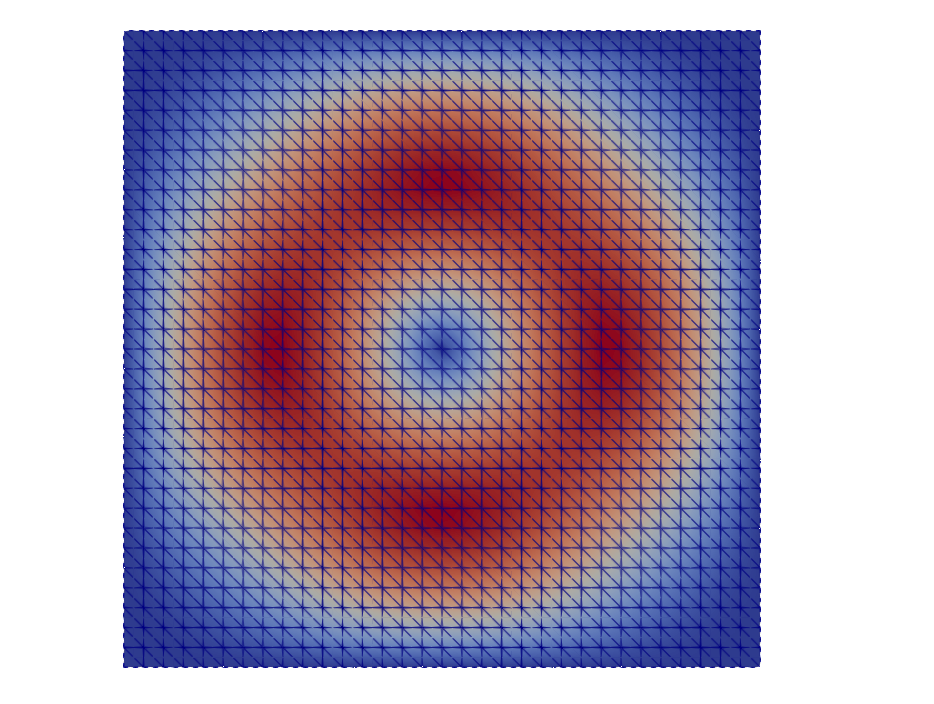
\includegraphics[scale=0.14]{Figures/P2P1DiscMesh.png}
			\qquad
			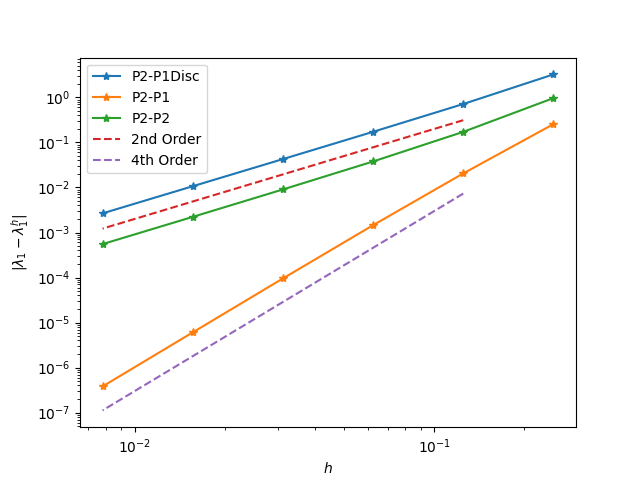
\includegraphics[scale=0.31]{Figures/P2P1Disc.png}
		\end{figure}
	\end{frame}
	\begin{frame}[fragile]
		\frametitle{Finite Element Exterior Calculus}
		\[
		\begin{tikzcd}
			0 \arrow{r} & H^2_0(\Omega) \arrow[d] \arrow{r}{\nabla\, \times} & \Big[H^1_0(\Omega)\Big]^2 \arrow[d] \arrow{r}{\nabla\,\cdot}& \mathcal{L}^2_0(\Omega)\arrow[d]  \arrow{r}& 0\\
			& \Sigma_h\arrow[d]  & \Phi_h \arrow{d}& \Xi_h \arrow{d}\\
			0 \arrow{r} & \Sigma_h \arrow{r}{\nabla\, \times} & \Phi_h \arrow{r}{\nabla\,\cdot}& \Xi_h^* \arrow{r}& 0
		\end{tikzcd}
		\]
	\end{frame}
	\begin{frame}
		\frametitle{Couple more example}	
		$\newline$
		\begin{itemize}
			\item [\color{oxfordblue}$\blacktriangleright$] $[\mathbb{P}^4(\mathcal{T}_h) ]^2 \; - \; \mathbb{P}^3_{disc}(\mathcal{T}_h)$, will be a converging scheme on a criss-cross mesh even if this choice of the element is not inf-sup stable.
			Best approximation estimates can be derived from the Morgan-Scott-Vogelius complex.
			\begin{figure}[h]
				\label{fig:DoF}
				$\newline$
				\centering
				\scalebox{0.45}{\tikzfig{Figures/DoF}}
			\end{figure}
		\end{itemize}
	\end{frame} 
	\begin{frame}
		\frametitle{Couple more example}	
		$\newline$
		\begin{itemize}
			\item [\color{oxfordblue}$\blacktriangleright$] $[\mathbb{P}^2(\mathcal{T}_h) ]^2 \; - \; \mathbb{P}^2(\mathcal{T}_h)$, will be a converging scheme on a barycentrically refined mesh even if this choice of the element is not inf-sup stable.
			Best approximation estimates can be derived from Hsieh-Clough-Tocher complex.
			\begin{figure}[h]
				\label{fig:DoF}
				$\newline$
				\centering
				\scalebox{0.45}{\tikzfig{Figures/DoF3}}
			\end{figure}
		\end{itemize}
	\end{frame} 
	\begin{frame}
		\frametitle{Conclusions}
		$\newline$
		$\newline$
		\begin{minipage}{5cm}
			\begin{itemize}
				\item<1->[\color{oxfordblue}$\blacktriangleright$] There is no need to characterise the range of the divergence operator! \textbf{\color{oxfordblue} This is crucial for three-dimensional problems.}
				\item<2->[\color{oxfordblue}$\blacktriangleright$] A wide variety of finite element space pairs can be used even if they are not \textbf{\color{oxfordblue} inf-sup} stable.
			\end{itemize}
		\end{minipage}
		\begin{minipage}{5cm}
			\begin{figure}
				\centering
				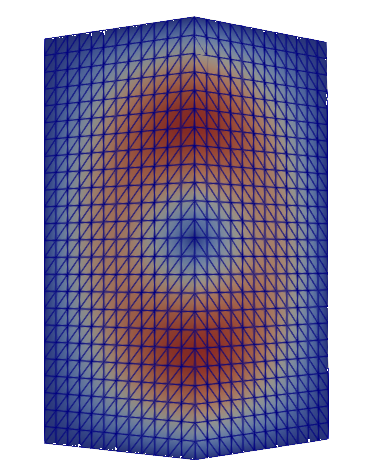
\includegraphics[scale=0.23]{Figures/3D.png}
			\end{figure}
		\end{minipage}
		$\newline$
		\visible<3->{
			\begin{center}
				\textbf{\color{oxfordblue} Thank you for your attention !}
			\end{center}
		}
	\end{frame}
\end{document}

\beamertemplatenavigationsymbolsempty
\let\vec\mathbf
\newcommand{\norm}[1]{\left\lVert#1\right\rVert}
\newcommand{\abs}[1]{\left|#1\right|}
\DeclareMathOperator{\Forall}{\forall}


%% Title slide formatting %%

\pgfdeclareimage[width=\paperwidth]{titlebackground}{Images/title-slide-background.png}
\setbeamerfont{subtitle}{size=\tiny}
\setbeamertemplate{endpage}{
	\begin{picture}(0,0)
		\scalebox{1.01}{
		\put(-28.5,-163){%
			\pgfuseimage{titlebackground}
		}
		}
		\put(0,-115){%
			\begin{minipage}[b][4.5cm][t]{0.5\textwidth}
				\color{white}
				\usebeamerfont{title}
				{\textbf{Thank Your} \\ \textbf{For You Attention !}}
			\end{minipage}
		}
	\end{picture}
}
\setbeamertemplate{title page}{
	\begin{picture}(0,0)
		\scalebox{1.01}{
			\put(-28.5,-163){%
				\pgfuseimage{titlebackground}
			}
		}
		\put(0,-75){%
			\begin{minipage}[b][4.5cm][t]{0.7\textwidth}
				\color{white}
				\usebeamerfont{title}
				{\inserttitle\\[0.9cm]}
				\usebeamerfont{subtitle}
				{\insertauthor\par}
				{\insertinstitute\\[0.3cm]}
				{\insertdate}
			\end{minipage}
		}
	\end{picture}
}


%% General slide formatting %%

\definecolor{oxfordblue}{RGB}{4,30,66}

\pgfdeclareimage[width=0.9cm]{oxfordlogo}{Images/oxford-logo.png}
\pgfdeclareimage[width=1cm]{mathslogo}{Images/mathematics-logo.png}
\pgfdeclareimage[width=0.9cm]{pizzalogo}{Images/pizza-logo.png}

\setbeamertemplate{headline}
{%
	\begin{picture}(0,0)
		\put(314,-50){%
			\pgfuseimage{oxfordlogo}
		}
		\put(20,-55){%
			\rule{320pt}{0.4pt}
		}
	\end{picture}
}

\setbeamertemplate{frametitle}
{%
	\begin{picture}(0,0)
		\put(-8,-20){%
			\normalsize\textbf{\color{oxfordblue}\insertframetitle}
		}
		\put(-7,-25){%
			\small\color{oxfordblue}\insertframesubtitle
		}
	\end{picture}
}

\setbeamertemplate{footline}
{%
	\begin{picture}(0,0)
		\put(20,30){%
			\rule{320pt}{0.4pt}
		}
		\put(20,14){%
			\pgfuseimage{mathslogo}
		}
		\put(100,14){%
			\color{oxfordblue}\insertshortdate
		}
		\put(160,14){%
			\color{oxfordblue}\insertshorttitle
		}
		\put(337,14){%
			\color{oxfordblue}\insertframenumber
		}
	\end{picture}%
}
\setbeamercolor{block title}{bg=oxfordblue!30,fg=black}

\definecolor{codegreen}{rgb}{0,0.6,0}
\definecolor{codegray}{rgb}{0.5,0.5,0.5}
\definecolor{codepurple}{rgb}{0.58,0,0.82}
\definecolor{backcolour}{rgb}{0.95,0.95,0.92}

\lstdefinestyle{mystyle}{
	%backgroundcolor=\color{backcolour},   
	commentstyle=\color{codegray},
	keywordstyle=\color{oxfordblue},
	numberstyle=\tiny\color{codegray},
	stringstyle=\color{codegreen},
	basicstyle=\ttfamily\footnotesize,
	breakatwhitespace=false,         
	breaklines=true,                 
	captionpos=b,                    
	keepspaces=true,                 
	numbers=left,                    
	numbersep=5pt,                  
	showspaces=false,                
	showstringspaces=false,
	showtabs=false,                  
	tabsize=2
}

\lstset{style=mystyle}

%% Information (author, title, etc.) %%

\title[Divergence-free discretisations of the Stokes eigenvalue problem]{Divergence-free discretisations of the Stokes eigenvalue problem} % short title for footer
\author%
{%
	\sc{Fleurianne Bertrand}\;*, \sc{Daniele Boffi}$\;\dagger$, \underline{\sc{U. Zerbinati}}$\;\ddagger$\\
}
\institute%
{%
	* \textit{Chemnitz University of Technology}
	\\
	$\;\dagger\;$\textit{King Abdullah University of Science and Technology}
	\\
	$\;\ddagger\;$\textit{University of Oxford}
}

\date[EFEF 2023]{European Finite Element Fair, 12th of May 2023\\ \\
\texttt{https://github.com/UZerbinati/EFEF2023}} % short date for footer



%% Content of slides %%

\begin{document}
	\begin{frame}[plain]
		\titlepage
	\end{frame}
	\begin{frame}
		\frametitle{Stokes eigenvalue problem}
		Find $(\vec{u},p)\!\in\!C^2_{0}(\Omega)\!\times\!\big[C^1(\Omega)\backslash \mathbb{R}\big]$ such that: 
		\begin{align}
			\nu\Delta \vec{u} - \nabla p &= \lambda \vec{u}\nonumber\\
			\nabla\cdot \vec{u} &= 0\nonumber
		\end{align}
		\begin{itemize}
			\item<2->[\color{oxfordblue}$\blacktriangleright$] The Stokes flow is characterized by advective inertial forces extremely small compared with viscous forces. 
			\item<3->[\color{oxfordblue}$\blacktriangleright$] Stokes flow can be used to model lubrication and viscous colloidal suspensions.
		\end{itemize}
	\end{frame}
	\begin{frame}
		\frametitle{The applications}
		\begin{itemize}
			\item [\color{oxfordblue}$\blacktriangleright$] The eigenfunctions of the Stokes eigenproblem span the space where solutions of the full Navier-Stokes equations are sought. 
		\end{itemize}
		$\newline$
		\begin{minipage}{0.45\textwidth}
			\begin{itemize}
				\item<2->[\color{oxfordblue}$\blacktriangleright$] The eigenvalues of the Stokes eigenproblem play a crucial role in computing a critical value for the Raynolds number, above which we will predict instabilities in Coutte flow.
			\end{itemize}
		\end{minipage}
		\qquad
		\begin{minipage}{0.45\textwidth}
			\visible<2->{
			\begin{figure}
				\centering
				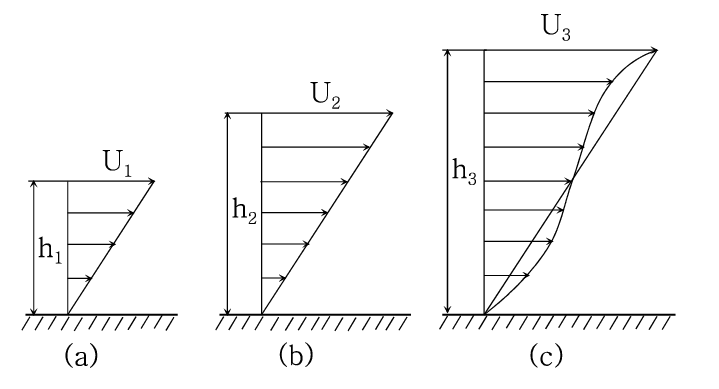
\includegraphics[scale=0.2]{Figures/Couette}
			\end{figure}
			}
		\end{minipage}
	\end{frame}
	\begin{frame}
		\frametitle{Our contribution}
		\begin{itemize}
			\item<1->[\color{oxfordblue}$\blacktriangleright$] We analyze divergence-free discretisations for the Stokes eigenvalue problem, and prove their well-posedness \textbf{\color{oxfordblue}independently} from the \textbf{\color{oxfordblue}characterization} of \textbf{\color{oxfordblue}the range} of the \textbf{\color{oxfordblue}discrete divergence operator}. 
			\item<2>[\color{oxfordblue}$\blacktriangleright$] We develop a systematic approach to \textbf{\color{oxfordblue}best approximation estimates} for functions living in the \textbf{\color{oxfordblue}kernel} of the \textbf{\color{oxfordblue}discrete divergence operator}, using \textbf{\color{oxfordblue}finite element exterior calculus}.
		\end{itemize}
	\end{frame}
	\begin{frame}
		\frametitle{Weak Stokes eigenvalue problem}
		$\newline$ 
		Find $(\vec{u},p)\!\in\!H^1_{0}(\Omega)\!\times\!\mathcal{L}^2_0(\Omega)$ such that $\Forall (\vec{v},q)\!\in\!H^1_0(\Omega)\!\times\!\mathcal{L}^2_0(\Omega)$,
		\begin{align*}
				\nu(\nabla \vec{u},\nabla \vec{v})_{\mathcal{L}^2(\Omega)}-(\nabla\cdot \vec{v},p)_{\mathcal{L}^2(\Omega)}&=\lambda_n\; (\vec{u},\vec{v})_{\mathcal{L}^2(\Omega)},\\
				(\nabla \cdot \vec{u}, q)_{\mathcal{L}^2(\Omega)} &= 0, 
		\end{align*}
		with $\lambda_n\in \mathbb{C}$, and $\nu\in \mathbb{R}_{> 0}$ is the fluid viscosity. 
		$\newline$
		\begin{itemize}
			\item<2->[\color{oxfordblue}$\blacktriangleright$] Are the eigenvalue of this problem real?
			\item<3->[\color{oxfordblue}$\blacktriangleright$] Do the eigenvalue of this problem diverge?
		\end{itemize}
	\end{frame}
	\begin{frame}
		\frametitle{Weak Stokes eigenvalue problem -- Laplace form}
		$\newline$ 
		$\newline$ 
		We introduce the space $H^1_{0,0}(\Omega)=\Big\{\vec{v}\in H^1_0(\Omega) \;:\; \nabla\cdot \vec{u} = 0 \Big\}$.
		\\
		$\newline$
		Find $\vec{u}\!\in\!H^1_{0,0}(\Omega)$ such that $\Forall \vec{v}\!\in\!H^1_{0,0}(\Omega)$,
		\begin{equation*}
				\nu(\nabla \vec{u},\nabla \vec{v})_{\mathcal{L}^2(\Omega)}=\lambda_n \;(\vec{u},\vec{v})_{\mathcal{L}^2(\Omega)},\label{eq:}
		\end{equation*}
		with $\lambda_n\in \mathbb{C}$, and $\nu\in \mathbb{R}_{> 0}$ is the fluid viscosity. 
		\vspace{0.2cm}
		\begin{itemize}
			\item<2->[\color{oxfordblue}$\blacktriangleright$] The eigenvalue problem is self-adjoint therefore $\lambda_n\in \mathbb{R}$.
			\item<3->[\color{oxfordblue}$\blacktriangleright$] $H^1_{0,0}(\Omega)$ is compactly embedded in $\mathcal{L}^2(\Omega)$ and therefore operator corresponding to the eigenvalue problem is compact, implying $\lambda_n \to \infty$ as $n\to\infty$.
		\end{itemize}
	\end{frame}
	\begin{frame}
		\frametitle{Discrete weak Stokes eigenvalue problem}
		$\newline$
		$\newline$
		$\newline$
		Find $(\vec{u}^h,p^h)\!\in\!V_h\!\times\!Q_h$ such that $\Forall\,(\vec{v}^h,q^h)\in V_h\times Q_h$,
		\begin{align*}
				\nu(\nabla \vec{u}^h,\nabla \vec{v}^h)_{\mathcal{L}^2(\Omega)}-(\nabla\cdot \vec{v}^h,p^h)_{\mathcal{L}^2(\Omega)}&=\lambda_n\; (\vec{u}^h,\vec{v}^h)_{\mathcal{L}^2(\Omega)},\\
				(\nabla \cdot \vec{u}^h, q^h)_{\mathcal{L}^2(\Omega)}&= 0, 
		\end{align*}
		with $\lambda_n^h\in \mathbb{C}$, $\nu\in \mathbb{R}_{> 0}$ is the fluid viscosity, and 
		\begin{equation*}
			\boxed{
				V_h\!\times\! Q_h \!\subset \!H^1_0(\Omega)\!\times\!\mathcal{L}^2_0(\Omega).
			}
		\end{equation*}
		\vspace{-0.5cm}
		\visible<2->{
			\begin{center}
				\color{oxfordblue} \textbf{Under what hypotheses on $V_h$ and $Q_h$ is  this eigenvalue problem well-posed ?}
			\end{center}
		}
	\end{frame}
	\begin{frame}{Babu\v{s}ka--Banach--Brezzi condition}
		\begin{columns}[T] 
			\begin{column}{0.65\textwidth} 
			
			\vspace{0.2cm} 
			\begin{block}{\textbf{\color{oxfordblue} Inf-Sup}}
				The \textbf{\color{oxfordblue}necessary} and \textbf{\color{oxfordblue}sufficient} condition for the well-posedness of the \textbf{\color{oxfordblue}source} problem is given by the \textbf{\color{oxfordblue}inf-sup} condition, i.e.
				\begin{equation}
					\underset{p_h \in Q_h}{\inf}\;\;\underset{\vec{v}_h\in V_h}{\sup} \frac{(\nabla\cdot v_h,p_h)_{\mathcal{L}^2(\Omega)}}{\norm{\vec{v}_h}_{H^1(\Omega)}\norm{p_h}_{\mathcal{L}^2(\Omega)}}\geq \beta,\nonumber 
				\end{equation}
				where $\beta$ ideally is independent of $h$.
			\end{block}
			\end{column} 
			
			\begin{column}{0.35\textwidth} 
				\vspace{1cm}
				\begin{figure} 
					\centering 
					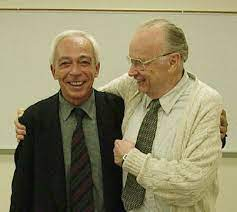
\includegraphics[width=1\textwidth]{Figures/BBB.jpeg} 
					\caption*{\tiny{F. Brezzi and I. Babu\v{s}ka}} 
				\end{figure} 
			\end{column} 
		\end{columns} 
	\end{frame}
	\begin{frame}{Boffi-Brezzi-Gastaldi observation}
		\begin{columns}[T] 
			\begin{column}{0.65\textwidth} 
			
			\vspace{0.2cm} 
			\begin{alertblock}{\textbf{Necessary and sufficient conditions}}
				When it comes to the eigenvalue problem, the inf-sup condition is \textbf{neither necessary nor sufficient}.
			\end{alertblock}
			\visible<2->{
				\begin{block}{\textbf{\color{oxfordblue}Q1-P0 Example}}
					Boffi, Brezzi and Gastaldi, showed that the \textbf{\color{oxfordblue} Q1-P0} finite element pair will lead to a converging eigenvalue problem, even if for this choice of element pair $\beta(h)\searrow 0$ as $h\to 0$.
				\end{block}
			}
			\end{column} 
			
			\begin{column}{0.35\textwidth} 
				\begin{figure} 
					\centering 
					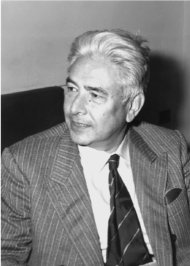
\includegraphics[width=0.8\textwidth]{Figures/DeGiorgi.jpg} 
					\caption*{\tiny{Enio De Giorgi, 1928--1996}} 
				\end{figure} 
			\end{column} 
		\end{columns} 
	\end{frame}
	\begin{frame}
		\frametitle{Boffi--Brezzi--Gastaldi conditions for Stokes}
		$\newline$
		\begin{itemize}
			\item<1->[\color{oxfordblue}$\blacktriangleright$] We say that $Q_h$ verifies the \textbf{\color{oxfordblue}weak approximability condition} if there exists $\gamma_1(h)$, such that for every $q \in \mathcal{L}^2_0(\Omega)$
				\begin{equation*}
					\underset{\vec{v}^h \in \mathbb{K}_h}{\sup} \frac{(\nabla\cdot\vec{v}^h,q)}{\norm{\vec{v}_h}_{H^1(\Omega)}} \leq \omega_1(h) \norm{q}_{\mathcal{L}^2(\Omega)} \; and \; \underset{h\to 0}{\lim}\,\gamma_1(h)=0.
				\end{equation*}
			\item<2->[\color{oxfordblue}$\blacktriangleright$] We say $V_h$ verifies the \textbf{\color{oxfordblue}strong approximability condition} if there exists $\gamma_2(h)$, such that for every $\vec{v} \in H^1_{0,0}(\Omega)\cap H^2(\Omega)$ 
				\begin{equation*}
					\underset{\vec{v}^h \in \mathbb{K}_h}{\inf} \norm{\vec{v}-\vec{v}^h}_{H^1(\Omega)} \leq \gamma_2(h)\norm{\vec{v}}_{H^2(\Omega)}\; and \; \underset{h\to 0}{\lim}\,\gamma_2(h)=0.
				\end{equation*}
		\end{itemize}
	\end{frame}
	\begin{frame}
		\frametitle{The divergence-free constraint}
		$\newline$
		$\newline$
		\begin{equation*}
			\boxed{
				b(\vec{v}^h,q^h)=(\nabla \cdot \vec{v}^h, q^h)_{\mathcal{L}^2(\Omega)}=0	
			}
		\end{equation*}
		$\newline$
		\visible<2->{
			Find $\vec{u}_h\!\in\!\mathbb{K}_{h}$ such that $\Forall \vec{v}_h\!\in\!\mathbb{K}_{h}$,
			\begin{equation*}
					\nu(\nabla \vec{u}^h,\nabla \vec{v}^h)_{\mathcal{L}^2(\Omega)}=\lambda_n^h \;(\vec{u}^h,\vec{v}^h)_{\mathcal{L}^2(\Omega)},
			\end{equation*}
			with $\lambda_n\in \mathbb{C}$, $\nu\in \mathbb{R}_{> 0}$ is the fluid viscosity and 
			\begin{equation*}
				\mathbb{K}_h=\Big\{\vec{v}^h\in V_h \;:\; b(\vec{v}^h,q^h) = 0, \Forall q^h\!\in\!Q_h\Big\}.
			\end{equation*}
		}
		\vspace{-0.3cm}
		\visible<3->{
			\begin{equation*}
				\boxed{\mathbb{K}_h\not\subset H^1_{0,0}(\Omega)}
			\end{equation*}
		}
	\end{frame}
	\begin{frame}
		\frametitle{Divergence-free discretisations}
		$\newline$
		\begin{equation*}
			\boxed{\nabla\cdot V_h\subset Q_h}
		\end{equation*}
		$\newline$
		\visible<2->{
			Under this hypothesis, we have the following result, i.e.
			\begin{equation*}
				b(\vec{v}^h,q^h)=(\nabla \cdot \vec{v}^h, q^h)_{\mathcal{L}^2(\Omega)}=0	\Leftrightarrow \nabla\cdot \vec{v}^h=0,
			\end{equation*}
			which implies the functions are point-wise \textbf{\color{oxfordblue}divergence-free}.
		}
		\visible<3->{
		\begin{equation*}
			\boxed{\mathbb{K}_h\subset H^1_{0,0}(\Omega)}
		\end{equation*}
		}
	\end{frame}
	\begin{frame}
		\frametitle{Divergence discretisations eigenvalue problem}
		$\newline$
		Find $\vec{u}_h\!\in\!\mathbb{K}_{h}$ such that $\Forall \vec{v}_h\!\in\mathbb{K}_{h}$,
		\begin{equation*}
				\nu(\nabla \vec{u}^h,\nabla \vec{v}^h)_{\mathcal{L}^2(\Omega)}=\lambda_n^h \;(\vec{u}^h,\vec{v}^h)_{\mathcal{L}^2(\Omega)},\label{eq:}
		\end{equation*}
		with $\nabla\cdot V_h\subset Q_h$, $\lambda_n\in \mathbb{C}$, $\nu\in \mathbb{R}_{> 0}$ is the fluid viscosity. 
		$\newline$
		\visible<2->{
			\begin{center}
				\color{oxfordblue} \textbf{This problem is well-posed and we can analyse it using Babu\v{s}ka-Osborn theory.}
			\end{center}
		}
	\end{frame}
	\begin{frame}
		\frametitle{Babu\v{s}ka--Osborn theory}
		\vspace{0.5cm}
		\begin{theorem}
			For each $n\in \mathbb{N}$, we have
			\begin{equation*}
				\lambda_n\leq \lambda_n^h \leq \lambda_n+C\underset{\vec{u}\in E,\;|\!|\vec{u}|\!|=1}{\sup}\;\underset{\vec{v}^h\in \mathbb{K}_{h}}{\inf}|\!| \vec{u}-\vec{v}_h |\!|_{H^{1}(\Omega)}^2
			\end{equation*}
			and there exists $\vec{w}^h_n\in \langle \vec{u}_{n}^h,\dots,\vec{u}_{n+m-1}^h\rangle$ such that
			\begin{equation*}
				|\!|\vec{u}_n-\vec{w}^h_n|\!|\leq C\underset{\vec{u}\in E,\;|\!|\vec{u}|\!|=1}{\sup}\;\underset{\vec{v}^h\in \mathbb{K}_{h}}{\inf}|\!| \vec{u}-\vec{v}_h |\!|_{H^{1}(\Omega)}
			\end{equation*}
			where $m$, $E$ and $\vec{u}_n$ are respectively the multiplicity, eigenspace and eigenvector corresponding to the eigenvalue $\lambda_n$.
		\end{theorem}
	\end{frame}
	\begin{frame}
		\frametitle{An example -- Type I mesh}
		\begin{lemma}
			Let $\vec{u} \in H^s(\Omega)\cap H^{1}_{0,0}(\Omega)$, with $s\geq 2$. On a special mesh obtained from a uniform square mesh dividing each cell along one of its diagonals there exists a $\vec{u}^h \in [\mathbb{P}^k(\mathcal{T}_h) ]^2$ such that
			\begin{align*}
				&\nabla\cdot \vec{u}_h = 0, \\
				&\norm{\vec{u}-\vec{u}_h}_{H^1(\Omega)} \leq C\abs{\vec{u}}_{H^s(\Omega)}\cdot \begin{cases}
					h^{\min(k-1,s-1)},\;\;\qquad k\in \{1,2,3\}\\
					h^{\min(k,s-1)}k^{(1-s)},\;\;\; k \geq 4
				\end{cases}
			\end{align*}
		\end{lemma}
	\end{frame}
	\begin{frame}
		\frametitle{An example -- Type I mesh}
		$\newline$
		\begin{equation*}
			\boxed{
				[\mathbb{P}^2(\mathcal{T}_h) ]^2 \; - \; \mathbb{P}^1_{disc}(\mathcal{T}_h) 
			}
		\end{equation*}
		\begin{figure}
			\centering
			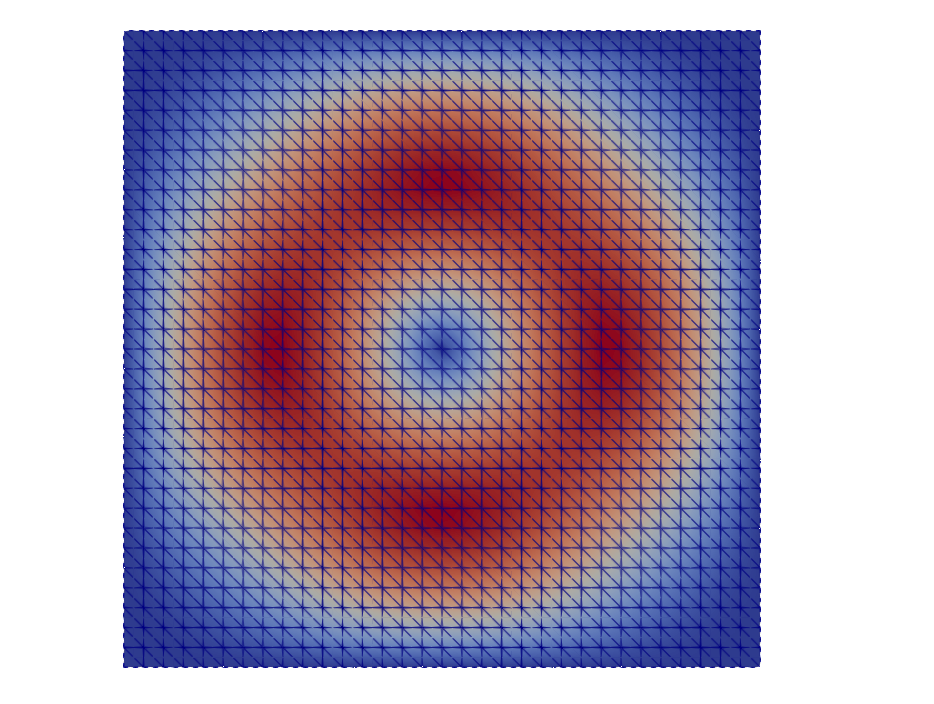
\includegraphics[scale=0.14]{Figures/P2P1DiscMesh.png}
			\qquad
			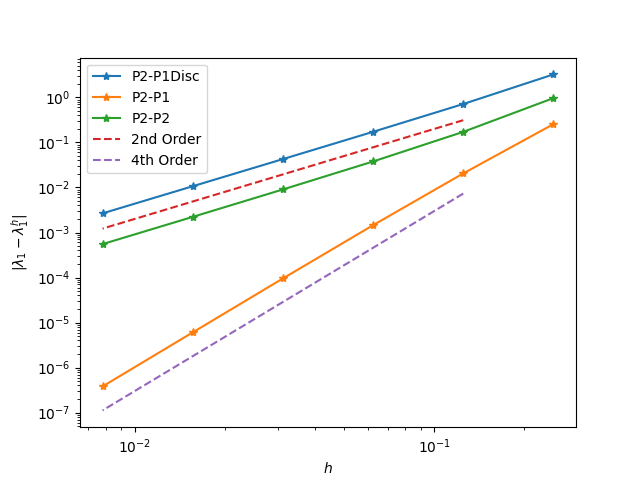
\includegraphics[scale=0.31]{Figures/P2P1Disc.png}
		\end{figure}
	\end{frame}
	\begin{frame}[fragile]
		\frametitle{Finite Element Exterior Calculus}
		\[
		\begin{tikzcd}
			0 \arrow{r} & H^2_0(\Omega) \arrow[d] \arrow{r}{\nabla\, \times} & \Big[H^1_0(\Omega)\Big]^2 \arrow[d] \arrow{r}{\nabla\,\cdot}& \mathcal{L}^2_0(\Omega)\arrow[d]  \arrow{r}& 0\\
			& \Sigma_h\arrow[d]  & \Phi_h \arrow{d}& \Xi_h \arrow{d}\\
			0 \arrow{r} & \Sigma_h \arrow{r}{\nabla\, \times} & \Phi_h \arrow{r}{\nabla\,\cdot}& \Xi_h^* \arrow{r}& 0
		\end{tikzcd}
		\]
	\end{frame}
	\begin{frame}
		\frametitle{Couple more example}	
		$\newline$
		\begin{itemize}
			\item [\color{oxfordblue}$\blacktriangleright$] $[\mathbb{P}^4(\mathcal{T}_h) ]^2 \; - \; \mathbb{P}^3_{disc}(\mathcal{T}_h)$, will be a converging scheme on a criss-cross mesh even if this choice of the element is not inf-sup stable.
			Best approximation estimates can be derived from the Morgan-Scott-Vogelius complex.
			\begin{figure}[h]
				\label{fig:DoF}
				$\newline$
				\centering
				\scalebox{0.45}{\tikzfig{Figures/DoF}}
			\end{figure}
		\end{itemize}
	\end{frame} 
	\begin{frame}
		\frametitle{Couple more example}	
		$\newline$
		\begin{itemize}
			\item [\color{oxfordblue}$\blacktriangleright$] $[\mathbb{P}^2(\mathcal{T}_h) ]^2 \; - \; \mathbb{P}^2(\mathcal{T}_h)$, will be a converging scheme on a barycentrically refined mesh even if this choice of the element is not inf-sup stable.
			Best approximation estimates can be derived from Hsieh-Clough-Tocher complex.
			\begin{figure}[h]
				\label{fig:DoF}
				$\newline$
				\centering
				\scalebox{0.45}{\tikzfig{Figures/DoF3}}
			\end{figure}
		\end{itemize}
	\end{frame} 
	\begin{frame}
		\frametitle{Conclusions}
		$\newline$
		$\newline$
		\begin{minipage}{5cm}
			\begin{itemize}
				\item<1->[\color{oxfordblue}$\blacktriangleright$] There is no need to characterise the range of the divergence operator! \textbf{\color{oxfordblue} This is crucial for three-dimensional problems.}
				\item<2->[\color{oxfordblue}$\blacktriangleright$] A wide variety of finite element space pairs can be used even if they are not \textbf{\color{oxfordblue} inf-sup} stable.
			\end{itemize}
		\end{minipage}
		\begin{minipage}{5cm}
			\begin{figure}
				\centering
				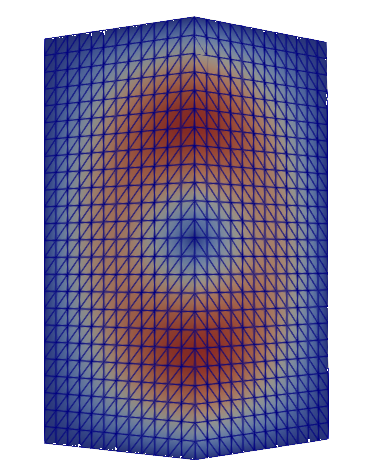
\includegraphics[scale=0.23]{Figures/3D.png}
			\end{figure}
		\end{minipage}
		$\newline$
		\visible<3->{
			\begin{center}
				\textbf{\color{oxfordblue} Thank you for your attention !}
			\end{center}
		}
	\end{frame}
\end{document}

\beamertemplatenavigationsymbolsempty
\let\vec\mathbf
\newcommand{\norm}[1]{\left\lVert#1\right\rVert}
\newcommand{\abs}[1]{\left|#1\right|}
\DeclareMathOperator{\Forall}{\forall}


%% Title slide formatting %%

\pgfdeclareimage[width=\paperwidth]{titlebackground}{Images/title-slide-background.png}
\setbeamerfont{subtitle}{size=\tiny}
\setbeamertemplate{endpage}{
	\begin{picture}(0,0)
		\scalebox{1.01}{
		\put(-28.5,-163){%
			\pgfuseimage{titlebackground}
		}
		}
		\put(0,-115){%
			\begin{minipage}[b][4.5cm][t]{0.5\textwidth}
				\color{white}
				\usebeamerfont{title}
				{\textbf{Thank Your} \\ \textbf{For You Attention !}}
			\end{minipage}
		}
	\end{picture}
}
\setbeamertemplate{title page}{
	\begin{picture}(0,0)
		\scalebox{1.01}{
			\put(-28.5,-163){%
				\pgfuseimage{titlebackground}
			}
		}
		\put(0,-75){%
			\begin{minipage}[b][4.5cm][t]{0.7\textwidth}
				\color{white}
				\usebeamerfont{title}
				{\inserttitle\\[0.9cm]}
				\usebeamerfont{subtitle}
				{\insertauthor\par}
				{\insertinstitute\\[0.3cm]}
				{\insertdate}
			\end{minipage}
		}
	\end{picture}
}


%% General slide formatting %%

\definecolor{oxfordblue}{RGB}{4,30,66}

\pgfdeclareimage[width=0.9cm]{oxfordlogo}{Images/oxford-logo.png}
\pgfdeclareimage[width=1cm]{mathslogo}{Images/mathematics-logo.png}
\pgfdeclareimage[width=0.9cm]{pizzalogo}{Images/pizza-logo.png}

\setbeamertemplate{headline}
{%
	\begin{picture}(0,0)
		\put(314,-50){%
			\pgfuseimage{oxfordlogo}
		}
		\put(20,-55){%
			\rule{320pt}{0.4pt}
		}
	\end{picture}
}

\setbeamertemplate{frametitle}
{%
	\begin{picture}(0,0)
		\put(-8,-20){%
			\normalsize\textbf{\color{oxfordblue}\insertframetitle}
		}
		\put(-7,-25){%
			\small\color{oxfordblue}\insertframesubtitle
		}
	\end{picture}
}

\setbeamertemplate{footline}
{%
	\begin{picture}(0,0)
		\put(20,30){%
			\rule{320pt}{0.4pt}
		}
		\put(20,14){%
			\pgfuseimage{mathslogo}
		}
		\put(100,14){%
			\color{oxfordblue}\insertshortdate
		}
		\put(160,14){%
			\color{oxfordblue}\insertshorttitle
		}
		\put(337,14){%
			\color{oxfordblue}\insertframenumber
		}
	\end{picture}%
}
\setbeamercolor{block title}{bg=oxfordblue!30,fg=black}

\definecolor{codegreen}{rgb}{0,0.6,0}
\definecolor{codegray}{rgb}{0.5,0.5,0.5}
\definecolor{codepurple}{rgb}{0.58,0,0.82}
\definecolor{backcolour}{rgb}{0.95,0.95,0.92}

\lstdefinestyle{mystyle}{
	%backgroundcolor=\color{backcolour},   
	commentstyle=\color{codegray},
	keywordstyle=\color{oxfordblue},
	numberstyle=\tiny\color{codegray},
	stringstyle=\color{codegreen},
	basicstyle=\ttfamily\footnotesize,
	breakatwhitespace=false,         
	breaklines=true,                 
	captionpos=b,                    
	keepspaces=true,                 
	numbers=left,                    
	numbersep=5pt,                  
	showspaces=false,                
	showstringspaces=false,
	showtabs=false,                  
	tabsize=2
}

\lstset{style=mystyle}

%% Information (author, title, etc.) %%

\title[Divergence-free discretisations of the Stokes eigenvalue problem]{Divergence-free discretisations of the Stokes eigenvalue problem} % short title for footer
\author%
{%
	\sc{Fleurianne Bertrand}\;*, \sc{Daniele Boffi}$\;\dagger$, \underline{\sc{U. Zerbinati}}$\;\ddagger$\\
}
\institute%
{%
	* \textit{Chemnitz University of Technology}
	\\
	$\;\dagger\;$\textit{King Abdullah University of Science and Technology}
	\\
	$\;\ddagger\;$\textit{University of Oxford}
}

\date[EFEF 2023]{European Finite Element Fair, 12th of May 2023\\ \\
\texttt{https://github.com/UZerbinati/EFEF2023}} % short date for footer



%% Content of slides %%

\begin{document}
	\begin{frame}[plain]
		\titlepage
	\end{frame}
	\begin{frame}
		\frametitle{Stokes eigenvalue problem}
		Find $(\vec{u},p)\!\in\!C^2_{0}(\Omega)\!\times\!\big[C^1(\Omega)\backslash \mathbb{R}\big]$ such that: 
		\begin{align}
			\nu\Delta \vec{u} - \nabla p &= \lambda \vec{u}\nonumber\\
			\nabla\cdot \vec{u} &= 0\nonumber
		\end{align}
		\begin{itemize}
			\item<2->[\color{oxfordblue}$\blacktriangleright$] The Stokes flow is characterized by advective inertial forces extremely small compared with viscous forces. 
			\item<3->[\color{oxfordblue}$\blacktriangleright$] Stokes flow can be used to model lubrication and viscous colloidal suspensions.
		\end{itemize}
	\end{frame}
	\begin{frame}
		\frametitle{The applications}
		\begin{itemize}
			\item [\color{oxfordblue}$\blacktriangleright$] The eigenfunctions of the Stokes eigenproblem span the space where solutions of the full Navier-Stokes equations are sought. 
		\end{itemize}
		$\newline$
		\begin{minipage}{0.45\textwidth}
			\begin{itemize}
				\item<2->[\color{oxfordblue}$\blacktriangleright$] The eigenvalues of the Stokes eigenproblem play a crucial role in computing a critical value for the Raynolds number, above which we will predict instabilities in Coutte flow.
			\end{itemize}
		\end{minipage}
		\qquad
		\begin{minipage}{0.45\textwidth}
			\visible<2->{
			\begin{figure}
				\centering
				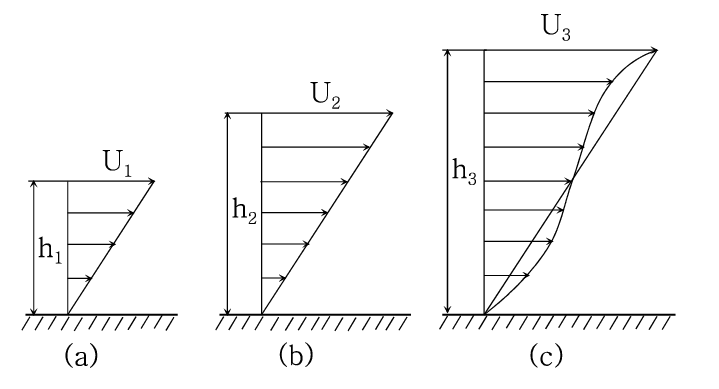
\includegraphics[scale=0.2]{Figures/Couette}
			\end{figure}
			}
		\end{minipage}
	\end{frame}
	\begin{frame}
		\frametitle{Our contribution}
		\begin{itemize}
			\item<1->[\color{oxfordblue}$\blacktriangleright$] We analyze divergence-free discretisations for the Stokes eigenvalue problem, and prove their well-posedness \textbf{\color{oxfordblue}independently} from the \textbf{\color{oxfordblue}characterization} of \textbf{\color{oxfordblue}the range} of the \textbf{\color{oxfordblue}discrete divergence operator}. 
			\item<2>[\color{oxfordblue}$\blacktriangleright$] We develop a systematic approach to \textbf{\color{oxfordblue}best approximation estimates} for functions living in the \textbf{\color{oxfordblue}kernel} of the \textbf{\color{oxfordblue}discrete divergence operator}, using \textbf{\color{oxfordblue}finite element exterior calculus}.
		\end{itemize}
	\end{frame}
	\begin{frame}
		\frametitle{Weak Stokes eigenvalue problem}
		$\newline$ 
		Find $(\vec{u},p)\!\in\!H^1_{0}(\Omega)\!\times\!\mathcal{L}^2_0(\Omega)$ such that $\Forall (\vec{v},q)\!\in\!H^1_0(\Omega)\!\times\!\mathcal{L}^2_0(\Omega)$,
		\begin{align*}
				\nu(\nabla \vec{u},\nabla \vec{v})_{\mathcal{L}^2(\Omega)}-(\nabla\cdot \vec{v},p)_{\mathcal{L}^2(\Omega)}&=\lambda_n\; (\vec{u},\vec{v})_{\mathcal{L}^2(\Omega)},\\
				(\nabla \cdot \vec{u}, q)_{\mathcal{L}^2(\Omega)} &= 0, 
		\end{align*}
		with $\lambda_n\in \mathbb{C}$, and $\nu\in \mathbb{R}_{> 0}$ is the fluid viscosity. 
		$\newline$
		\begin{itemize}
			\item<2->[\color{oxfordblue}$\blacktriangleright$] Are the eigenvalue of this problem real?
			\item<3->[\color{oxfordblue}$\blacktriangleright$] Do the eigenvalue of this problem diverge?
		\end{itemize}
	\end{frame}
	\begin{frame}
		\frametitle{Weak Stokes eigenvalue problem -- Laplace form}
		$\newline$ 
		$\newline$ 
		We introduce the space $H^1_{0,0}(\Omega)=\Big\{\vec{v}\in H^1_0(\Omega) \;:\; \nabla\cdot \vec{u} = 0 \Big\}$.
		\\
		$\newline$
		Find $\vec{u}\!\in\!H^1_{0,0}(\Omega)$ such that $\Forall \vec{v}\!\in\!H^1_{0,0}(\Omega)$,
		\begin{equation*}
				\nu(\nabla \vec{u},\nabla \vec{v})_{\mathcal{L}^2(\Omega)}=\lambda_n \;(\vec{u},\vec{v})_{\mathcal{L}^2(\Omega)},\label{eq:}
		\end{equation*}
		with $\lambda_n\in \mathbb{C}$, and $\nu\in \mathbb{R}_{> 0}$ is the fluid viscosity. 
		\vspace{0.2cm}
		\begin{itemize}
			\item<2->[\color{oxfordblue}$\blacktriangleright$] The eigenvalue problem is self-adjoint therefore $\lambda_n\in \mathbb{R}$.
			\item<3->[\color{oxfordblue}$\blacktriangleright$] $H^1_{0,0}(\Omega)$ is compactly embedded in $\mathcal{L}^2(\Omega)$ and therefore operator corresponding to the eigenvalue problem is compact, implying $\lambda_n \to \infty$ as $n\to\infty$.
		\end{itemize}
	\end{frame}
	\begin{frame}
		\frametitle{Discrete weak Stokes eigenvalue problem}
		$\newline$
		$\newline$
		$\newline$
		Find $(\vec{u}^h,p^h)\!\in\!V_h\!\times\!Q_h$ such that $\Forall\,(\vec{v}^h,q^h)\in V_h\times Q_h$,
		\begin{align*}
				\nu(\nabla \vec{u}^h,\nabla \vec{v}^h)_{\mathcal{L}^2(\Omega)}-(\nabla\cdot \vec{v}^h,p^h)_{\mathcal{L}^2(\Omega)}&=\lambda_n\; (\vec{u}^h,\vec{v}^h)_{\mathcal{L}^2(\Omega)},\\
				(\nabla \cdot \vec{u}^h, q^h)_{\mathcal{L}^2(\Omega)}&= 0, 
		\end{align*}
		with $\lambda_n^h\in \mathbb{C}$, $\nu\in \mathbb{R}_{> 0}$ is the fluid viscosity, and 
		\begin{equation*}
			\boxed{
				V_h\!\times\! Q_h \!\subset \!H^1_0(\Omega)\!\times\!\mathcal{L}^2_0(\Omega).
			}
		\end{equation*}
		\vspace{-0.5cm}
		\visible<2->{
			\begin{center}
				\color{oxfordblue} \textbf{Under what hypotheses on $V_h$ and $Q_h$ is  this eigenvalue problem well-posed ?}
			\end{center}
		}
	\end{frame}
	\begin{frame}{Babu\v{s}ka--Banach--Brezzi condition}
		\begin{columns}[T] 
			\begin{column}{0.65\textwidth} 
			
			\vspace{0.2cm} 
			\begin{block}{\textbf{\color{oxfordblue} Inf-Sup}}
				The \textbf{\color{oxfordblue}necessary} and \textbf{\color{oxfordblue}sufficient} condition for the well-posedness of the \textbf{\color{oxfordblue}source} problem is given by the \textbf{\color{oxfordblue}inf-sup} condition, i.e.
				\begin{equation}
					\underset{p_h \in Q_h}{\inf}\;\;\underset{\vec{v}_h\in V_h}{\sup} \frac{(\nabla\cdot v_h,p_h)_{\mathcal{L}^2(\Omega)}}{\norm{\vec{v}_h}_{H^1(\Omega)}\norm{p_h}_{\mathcal{L}^2(\Omega)}}\geq \beta,\nonumber 
				\end{equation}
				where $\beta$ ideally is independent of $h$.
			\end{block}
			\end{column} 
			
			\begin{column}{0.35\textwidth} 
				\vspace{1cm}
				\begin{figure} 
					\centering 
					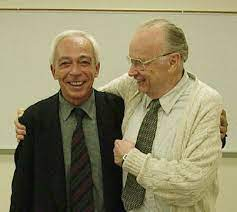
\includegraphics[width=1\textwidth]{Figures/BBB.jpeg} 
					\caption*{\tiny{F. Brezzi and I. Babu\v{s}ka}} 
				\end{figure} 
			\end{column} 
		\end{columns} 
	\end{frame}
	\begin{frame}{Boffi-Brezzi-Gastaldi observation}
		\begin{columns}[T] 
			\begin{column}{0.65\textwidth} 
			
			\vspace{0.2cm} 
			\begin{alertblock}{\textbf{Necessary and sufficient conditions}}
				When it comes to the eigenvalue problem, the inf-sup condition is \textbf{neither necessary nor sufficient}.
			\end{alertblock}
			\visible<2->{
				\begin{block}{\textbf{\color{oxfordblue}Q1-P0 Example}}
					Boffi, Brezzi and Gastaldi, showed that the \textbf{\color{oxfordblue} Q1-P0} finite element pair will lead to a converging eigenvalue problem, even if for this choice of element pair $\beta(h)\searrow 0$ as $h\to 0$.
				\end{block}
			}
			\end{column} 
			
			\begin{column}{0.35\textwidth} 
				\begin{figure} 
					\centering 
					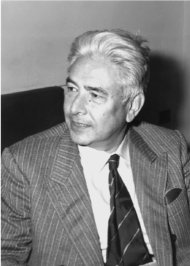
\includegraphics[width=0.8\textwidth]{Figures/DeGiorgi.jpg} 
					\caption*{\tiny{Enio De Giorgi, 1928--1996}} 
				\end{figure} 
			\end{column} 
		\end{columns} 
	\end{frame}
	\begin{frame}
		\frametitle{Boffi--Brezzi--Gastaldi conditions for Stokes}
		$\newline$
		\begin{itemize}
			\item<1->[\color{oxfordblue}$\blacktriangleright$] We say that $Q_h$ verifies the \textbf{\color{oxfordblue}weak approximability condition} if there exists $\gamma_1(h)$, such that for every $q \in \mathcal{L}^2_0(\Omega)$
				\begin{equation*}
					\underset{\vec{v}^h \in \mathbb{K}_h}{\sup} \frac{(\nabla\cdot\vec{v}^h,q)}{\norm{\vec{v}_h}_{H^1(\Omega)}} \leq \omega_1(h) \norm{q}_{\mathcal{L}^2(\Omega)} \; and \; \underset{h\to 0}{\lim}\,\gamma_1(h)=0.
				\end{equation*}
			\item<2->[\color{oxfordblue}$\blacktriangleright$] We say $V_h$ verifies the \textbf{\color{oxfordblue}strong approximability condition} if there exists $\gamma_2(h)$, such that for every $\vec{v} \in H^1_{0,0}(\Omega)\cap H^2(\Omega)$ 
				\begin{equation*}
					\underset{\vec{v}^h \in \mathbb{K}_h}{\inf} \norm{\vec{v}-\vec{v}^h}_{H^1(\Omega)} \leq \gamma_2(h)\norm{\vec{v}}_{H^2(\Omega)}\; and \; \underset{h\to 0}{\lim}\,\gamma_2(h)=0.
				\end{equation*}
		\end{itemize}
	\end{frame}
	\begin{frame}
		\frametitle{The divergence-free constraint}
		$\newline$
		$\newline$
		\begin{equation*}
			\boxed{
				b(\vec{v}^h,q^h)=(\nabla \cdot \vec{v}^h, q^h)_{\mathcal{L}^2(\Omega)}=0	
			}
		\end{equation*}
		$\newline$
		\visible<2->{
			Find $\vec{u}_h\!\in\!\mathbb{K}_{h}$ such that $\Forall \vec{v}_h\!\in\!\mathbb{K}_{h}$,
			\begin{equation*}
					\nu(\nabla \vec{u}^h,\nabla \vec{v}^h)_{\mathcal{L}^2(\Omega)}=\lambda_n^h \;(\vec{u}^h,\vec{v}^h)_{\mathcal{L}^2(\Omega)},
			\end{equation*}
			with $\lambda_n\in \mathbb{C}$, $\nu\in \mathbb{R}_{> 0}$ is the fluid viscosity and 
			\begin{equation*}
				\mathbb{K}_h=\Big\{\vec{v}^h\in V_h \;:\; b(\vec{v}^h,q^h) = 0, \Forall q^h\!\in\!Q_h\Big\}.
			\end{equation*}
		}
		\vspace{-0.3cm}
		\visible<3->{
			\begin{equation*}
				\boxed{\mathbb{K}_h\not\subset H^1_{0,0}(\Omega)}
			\end{equation*}
		}
	\end{frame}
	\begin{frame}
		\frametitle{Divergence-free discretisations}
		$\newline$
		\begin{equation*}
			\boxed{\nabla\cdot V_h\subset Q_h}
		\end{equation*}
		$\newline$
		\visible<2->{
			Under this hypothesis, we have the following result, i.e.
			\begin{equation*}
				b(\vec{v}^h,q^h)=(\nabla \cdot \vec{v}^h, q^h)_{\mathcal{L}^2(\Omega)}=0	\Leftrightarrow \nabla\cdot \vec{v}^h=0,
			\end{equation*}
			which implies the functions are point-wise \textbf{\color{oxfordblue}divergence-free}.
		}
		\visible<3->{
		\begin{equation*}
			\boxed{\mathbb{K}_h\subset H^1_{0,0}(\Omega)}
		\end{equation*}
		}
	\end{frame}
	\begin{frame}
		\frametitle{Divergence discretisations eigenvalue problem}
		$\newline$
		Find $\vec{u}_h\!\in\!\mathbb{K}_{h}$ such that $\Forall \vec{v}_h\!\in\mathbb{K}_{h}$,
		\begin{equation*}
				\nu(\nabla \vec{u}^h,\nabla \vec{v}^h)_{\mathcal{L}^2(\Omega)}=\lambda_n^h \;(\vec{u}^h,\vec{v}^h)_{\mathcal{L}^2(\Omega)},\label{eq:}
		\end{equation*}
		with $\nabla\cdot V_h\subset Q_h$, $\lambda_n\in \mathbb{C}$, $\nu\in \mathbb{R}_{> 0}$ is the fluid viscosity. 
		$\newline$
		\visible<2->{
			\begin{center}
				\color{oxfordblue} \textbf{This problem is well-posed and we can analyse it using Babu\v{s}ka-Osborn theory.}
			\end{center}
		}
	\end{frame}
	\begin{frame}
		\frametitle{Babu\v{s}ka--Osborn theory}
		\vspace{0.5cm}
		\begin{theorem}
			For each $n\in \mathbb{N}$, we have
			\begin{equation*}
				\lambda_n\leq \lambda_n^h \leq \lambda_n+C\underset{\vec{u}\in E,\;|\!|\vec{u}|\!|=1}{\sup}\;\underset{\vec{v}^h\in \mathbb{K}_{h}}{\inf}|\!| \vec{u}-\vec{v}_h |\!|_{H^{1}(\Omega)}^2
			\end{equation*}
			and there exists $\vec{w}^h_n\in \langle \vec{u}_{n}^h,\dots,\vec{u}_{n+m-1}^h\rangle$ such that
			\begin{equation*}
				|\!|\vec{u}_n-\vec{w}^h_n|\!|\leq C\underset{\vec{u}\in E,\;|\!|\vec{u}|\!|=1}{\sup}\;\underset{\vec{v}^h\in \mathbb{K}_{h}}{\inf}|\!| \vec{u}-\vec{v}_h |\!|_{H^{1}(\Omega)}
			\end{equation*}
			where $m$, $E$ and $\vec{u}_n$ are respectively the multiplicity, eigenspace and eigenvector corresponding to the eigenvalue $\lambda_n$.
		\end{theorem}
	\end{frame}
	\begin{frame}
		\frametitle{An example -- Type I mesh}
		\begin{lemma}
			Let $\vec{u} \in H^s(\Omega)\cap H^{1}_{0,0}(\Omega)$, with $s\geq 2$. On a special mesh obtained from a uniform square mesh dividing each cell along one of its diagonals there exists a $\vec{u}^h \in [\mathbb{P}^k(\mathcal{T}_h) ]^2$ such that
			\begin{align*}
				&\nabla\cdot \vec{u}_h = 0, \\
				&\norm{\vec{u}-\vec{u}_h}_{H^1(\Omega)} \leq C\abs{\vec{u}}_{H^s(\Omega)}\cdot \begin{cases}
					h^{\min(k-1,s-1)},\;\;\qquad k\in \{1,2,3\}\\
					h^{\min(k,s-1)}k^{(1-s)},\;\;\; k \geq 4
				\end{cases}
			\end{align*}
		\end{lemma}
	\end{frame}
	\begin{frame}
		\frametitle{An example -- Type I mesh}
		$\newline$
		\begin{equation*}
			\boxed{
				[\mathbb{P}^2(\mathcal{T}_h) ]^2 \; - \; \mathbb{P}^1_{disc}(\mathcal{T}_h) 
			}
		\end{equation*}
		\begin{figure}
			\centering
			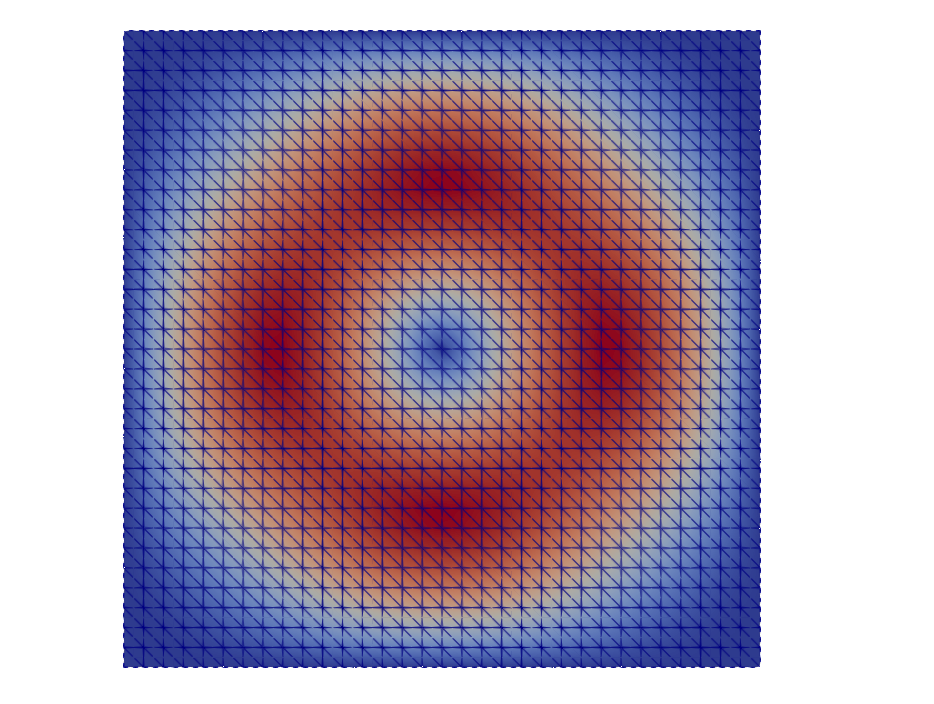
\includegraphics[scale=0.14]{Figures/P2P1DiscMesh.png}
			\qquad
			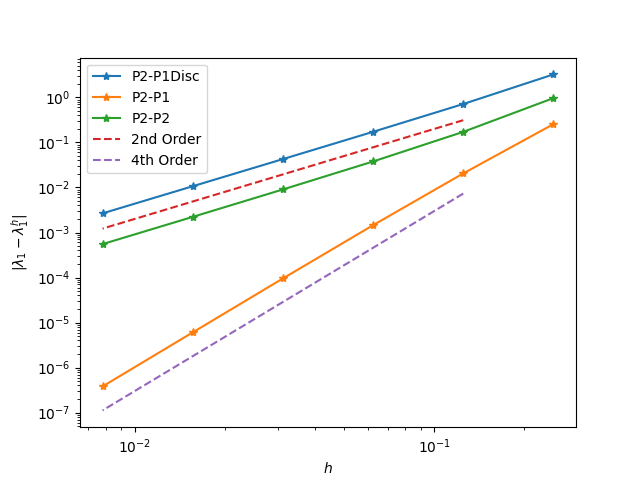
\includegraphics[scale=0.31]{Figures/P2P1Disc.png}
		\end{figure}
	\end{frame}
	\begin{frame}[fragile]
		\frametitle{Finite Element Exterior Calculus}
		\[
		\begin{tikzcd}
			0 \arrow{r} & H^2_0(\Omega) \arrow[d] \arrow{r}{\nabla\, \times} & \Big[H^1_0(\Omega)\Big]^2 \arrow[d] \arrow{r}{\nabla\,\cdot}& \mathcal{L}^2_0(\Omega)\arrow[d]  \arrow{r}& 0\\
			& \Sigma_h\arrow[d]  & \Phi_h \arrow{d}& \Xi_h \arrow{d}\\
			0 \arrow{r} & \Sigma_h \arrow{r}{\nabla\, \times} & \Phi_h \arrow{r}{\nabla\,\cdot}& \Xi_h^* \arrow{r}& 0
		\end{tikzcd}
		\]
	\end{frame}
	\begin{frame}
		\frametitle{Couple more example}	
		$\newline$
		\begin{itemize}
			\item [\color{oxfordblue}$\blacktriangleright$] $[\mathbb{P}^4(\mathcal{T}_h) ]^2 \; - \; \mathbb{P}^3_{disc}(\mathcal{T}_h)$, will be a converging scheme on a criss-cross mesh even if this choice of the element is not inf-sup stable.
			Best approximation estimates can be derived from the Morgan-Scott-Vogelius complex.
			\begin{figure}[h]
				\label{fig:DoF}
				$\newline$
				\centering
				\scalebox{0.45}{\tikzfig{Figures/DoF}}
			\end{figure}
		\end{itemize}
	\end{frame} 
	\begin{frame}
		\frametitle{Couple more example}	
		$\newline$
		\begin{itemize}
			\item [\color{oxfordblue}$\blacktriangleright$] $[\mathbb{P}^2(\mathcal{T}_h) ]^2 \; - \; \mathbb{P}^2(\mathcal{T}_h)$, will be a converging scheme on a barycentrically refined mesh even if this choice of the element is not inf-sup stable.
			Best approximation estimates can be derived from Hsieh-Clough-Tocher complex.
			\begin{figure}[h]
				\label{fig:DoF}
				$\newline$
				\centering
				\scalebox{0.45}{\tikzfig{Figures/DoF3}}
			\end{figure}
		\end{itemize}
	\end{frame} 
	\begin{frame}
		\frametitle{Conclusions}
		$\newline$
		$\newline$
		\begin{minipage}{5cm}
			\begin{itemize}
				\item<1->[\color{oxfordblue}$\blacktriangleright$] There is no need to characterise the range of the divergence operator! \textbf{\color{oxfordblue} This is crucial for three-dimensional problems.}
				\item<2->[\color{oxfordblue}$\blacktriangleright$] A wide variety of finite element space pairs can be used even if they are not \textbf{\color{oxfordblue} inf-sup} stable.
			\end{itemize}
		\end{minipage}
		\begin{minipage}{5cm}
			\begin{figure}
				\centering
				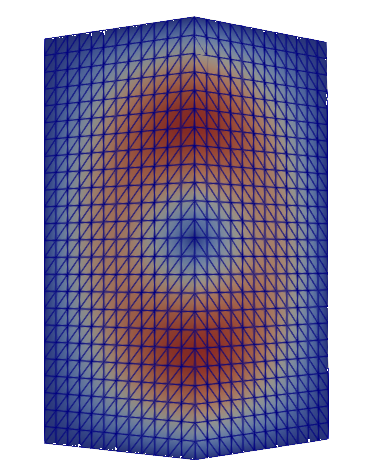
\includegraphics[scale=0.23]{Figures/3D.png}
			\end{figure}
		\end{minipage}
		$\newline$
		\visible<3->{
			\begin{center}
				\textbf{\color{oxfordblue} Thank you for your attention !}
			\end{center}
		}
	\end{frame}
\end{document}

\beamertemplatenavigationsymbolsempty
\let\vec\mathbf
\newcommand{\norm}[1]{\left\lVert#1\right\rVert}
\newcommand{\abs}[1]{\left|#1\right|}
\DeclareMathOperator{\Forall}{\forall}


%% Title slide formatting %%

\pgfdeclareimage[width=\paperwidth]{titlebackground}{Images/title-slide-background.png}
\setbeamerfont{subtitle}{size=\tiny}
\setbeamertemplate{endpage}{
	\begin{picture}(0,0)
		\scalebox{1.01}{
		\put(-28.5,-163){%
			\pgfuseimage{titlebackground}
		}
		}
		\put(0,-115){%
			\begin{minipage}[b][4.5cm][t]{0.5\textwidth}
				\color{white}
				\usebeamerfont{title}
				{\textbf{Thank Your} \\ \textbf{For You Attention !}}
			\end{minipage}
		}
	\end{picture}
}
\setbeamertemplate{title page}{
	\begin{picture}(0,0)
		\scalebox{1.01}{
			\put(-28.5,-163){%
				\pgfuseimage{titlebackground}
			}
		}
		\put(0,-75){%
			\begin{minipage}[b][4.5cm][t]{0.7\textwidth}
				\color{white}
				\usebeamerfont{title}
				{\inserttitle\\[0.9cm]}
				\usebeamerfont{subtitle}
				{\insertauthor\par}
				{\insertinstitute\\[0.3cm]}
				{\insertdate}
			\end{minipage}
		}
	\end{picture}
}


%% General slide formatting %%

\definecolor{oxfordblue}{RGB}{4,30,66}

\pgfdeclareimage[width=0.9cm]{oxfordlogo}{Images/oxford-logo.png}
\pgfdeclareimage[width=1cm]{mathslogo}{Images/mathematics-logo.png}
\pgfdeclareimage[width=0.9cm]{pizzalogo}{Images/pizza-logo.png}

\setbeamertemplate{headline}
{%
	\begin{picture}(0,0)
		\put(314,-50){%
			\pgfuseimage{oxfordlogo}
		}
		\put(20,-55){%
			\rule{320pt}{0.4pt}
		}
	\end{picture}
}

\setbeamertemplate{frametitle}
{%
	\begin{picture}(0,0)
		\put(-8,-20){%
			\normalsize\textbf{\color{oxfordblue}\insertframetitle}
		}
		\put(-7,-25){%
			\small\color{oxfordblue}\insertframesubtitle
		}
	\end{picture}
}

\setbeamertemplate{footline}
{%
	\begin{picture}(0,0)
		\put(20,30){%
			\rule{320pt}{0.4pt}
		}
		\put(20,14){%
			\pgfuseimage{mathslogo}
		}
		\put(100,14){%
			\color{oxfordblue}\insertshortdate
		}
		\put(160,14){%
			\color{oxfordblue}\insertshorttitle
		}
		\put(337,14){%
			\color{oxfordblue}\insertframenumber
		}
	\end{picture}%
}
\setbeamercolor{block title}{bg=oxfordblue!30,fg=black}

\definecolor{codegreen}{rgb}{0,0.6,0}
\definecolor{codegray}{rgb}{0.5,0.5,0.5}
\definecolor{codepurple}{rgb}{0.58,0,0.82}
\definecolor{backcolour}{rgb}{0.95,0.95,0.92}

\lstdefinestyle{mystyle}{
	%backgroundcolor=\color{backcolour},   
	commentstyle=\color{codegray},
	keywordstyle=\color{oxfordblue},
	numberstyle=\tiny\color{codegray},
	stringstyle=\color{codegreen},
	basicstyle=\ttfamily\footnotesize,
	breakatwhitespace=false,         
	breaklines=true,                 
	captionpos=b,                    
	keepspaces=true,                 
	numbers=left,                    
	numbersep=5pt,                  
	showspaces=false,                
	showstringspaces=false,
	showtabs=false,                  
	tabsize=2
}

\lstset{style=mystyle}

%% Information (author, title, etc.) %%

\title[Divergence-free discretisations of the Stokes eigenvalue problem]{Divergence-free discretisations of the Stokes eigenvalue problem} % short title for footer
\author%
{%
	\sc{Fleurianne Bertrand}\;*, \sc{Daniele Boffi}$\;\dagger$, \underline{\sc{U. Zerbinati}}$\;\ddagger$\\
}
\institute%
{%
	* \textit{Chemnitz University of Technology}
	\\
	$\;\dagger\;$\textit{King Abdullah University of Science and Technology}
	\\
	$\;\ddagger\;$\textit{University of Oxford}
}

\date[EFEF 2023]{European Finite Element Fair, 12th of May 2023\\ \\
\texttt{https://github.com/UZerbinati/EFEF2023}} % short date for footer



%% Content of slides %%

\begin{document}
	\begin{frame}[plain]
		\titlepage
	\end{frame}
	\begin{frame}
		\frametitle{Stokes eigenvalue problem}
		Find $(\vec{u},p)\!\in\!C^2_{0}(\Omega)\!\times\!\big[C^1(\Omega)\backslash \mathbb{R}\big]$ such that: 
		\begin{align}
			\nu\Delta \vec{u} - \nabla p &= \lambda \vec{u}\nonumber\\
			\nabla\cdot \vec{u} &= 0\nonumber
		\end{align}
		\begin{itemize}
			\item<2->[\color{oxfordblue}$\blacktriangleright$] The Stokes flow is characterized by advective inertial forces extremely small compared with viscous forces. 
			\item<3->[\color{oxfordblue}$\blacktriangleright$] Stokes flow can be used to model lubrication and viscous colloidal suspensions.
		\end{itemize}
	\end{frame}
	\begin{frame}
		\frametitle{The applications}
		\begin{itemize}
			\item [\color{oxfordblue}$\blacktriangleright$] The eigenfunctions of the Stokes eigenproblem span the space where solutions of the full Navier-Stokes equations are sought. 
		\end{itemize}
		$\newline$
		\begin{minipage}{0.45\textwidth}
			\begin{itemize}
				\item<2->[\color{oxfordblue}$\blacktriangleright$] The eigenvalues of the Stokes eigenproblem play a crucial role in computing a critical value for the Raynolds number, above which we will predict instabilities in Coutte flow.
			\end{itemize}
		\end{minipage}
		\qquad
		\begin{minipage}{0.45\textwidth}
			\visible<2->{
			\begin{figure}
				\centering
				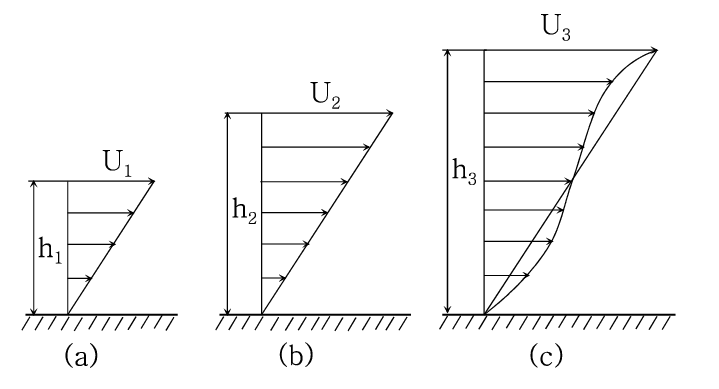
\includegraphics[scale=0.2]{Figures/Couette}
			\end{figure}
			}
		\end{minipage}
	\end{frame}
	\begin{frame}
		\frametitle{Our contribution}
		\begin{itemize}
			\item<1->[\color{oxfordblue}$\blacktriangleright$] We analyze divergence-free discretisations for the Stokes eigenvalue problem, and prove their well-posedness \textbf{\color{oxfordblue}independently} from the \textbf{\color{oxfordblue}characterization} of \textbf{\color{oxfordblue}the range} of the \textbf{\color{oxfordblue}discrete divergence operator}. 
			\item<2>[\color{oxfordblue}$\blacktriangleright$] We develop a systematic approach to \textbf{\color{oxfordblue}best approximation estimates} for functions living in the \textbf{\color{oxfordblue}kernel} of the \textbf{\color{oxfordblue}discrete divergence operator}, using \textbf{\color{oxfordblue}finite element exterior calculus}.
		\end{itemize}
	\end{frame}
	\begin{frame}
		\frametitle{Weak Stokes eigenvalue problem}
		$\newline$ 
		Find $(\vec{u},p)\!\in\!H^1_{0}(\Omega)\!\times\!\mathcal{L}^2_0(\Omega)$ such that $\Forall (\vec{v},q)\!\in\!H^1_0(\Omega)\!\times\!\mathcal{L}^2_0(\Omega)$,
		\begin{align*}
				\nu(\nabla \vec{u},\nabla \vec{v})_{\mathcal{L}^2(\Omega)}-(\nabla\cdot \vec{v},p)_{\mathcal{L}^2(\Omega)}&=\lambda_n\; (\vec{u},\vec{v})_{\mathcal{L}^2(\Omega)},\\
				(\nabla \cdot \vec{u}, q)_{\mathcal{L}^2(\Omega)} &= 0, 
		\end{align*}
		with $\lambda_n\in \mathbb{C}$, and $\nu\in \mathbb{R}_{> 0}$ is the fluid viscosity. 
		$\newline$
		\begin{itemize}
			\item<2->[\color{oxfordblue}$\blacktriangleright$] Are the eigenvalue of this problem real?
			\item<3->[\color{oxfordblue}$\blacktriangleright$] Do the eigenvalue of this problem diverge?
		\end{itemize}
	\end{frame}
	\begin{frame}
		\frametitle{Weak Stokes eigenvalue problem -- Laplace form}
		$\newline$ 
		$\newline$ 
		We introduce the space $H^1_{0,0}(\Omega)=\Big\{\vec{v}\in H^1_0(\Omega) \;:\; \nabla\cdot \vec{u} = 0 \Big\}$.
		\\
		$\newline$
		Find $\vec{u}\!\in\!H^1_{0,0}(\Omega)$ such that $\Forall \vec{v}\!\in\!H^1_{0,0}(\Omega)$,
		\begin{equation*}
				\nu(\nabla \vec{u},\nabla \vec{v})_{\mathcal{L}^2(\Omega)}=\lambda_n \;(\vec{u},\vec{v})_{\mathcal{L}^2(\Omega)},\label{eq:}
		\end{equation*}
		with $\lambda_n\in \mathbb{C}$, and $\nu\in \mathbb{R}_{> 0}$ is the fluid viscosity. 
		\vspace{0.2cm}
		\begin{itemize}
			\item<2->[\color{oxfordblue}$\blacktriangleright$] The eigenvalue problem is self-adjoint therefore $\lambda_n\in \mathbb{R}$.
			\item<3->[\color{oxfordblue}$\blacktriangleright$] $H^1_{0,0}(\Omega)$ is compactly embedded in $\mathcal{L}^2(\Omega)$ and therefore operator corresponding to the eigenvalue problem is compact, implying $\lambda_n \to \infty$ as $n\to\infty$.
		\end{itemize}
	\end{frame}
	\begin{frame}
		\frametitle{Discrete weak Stokes eigenvalue problem}
		$\newline$
		$\newline$
		$\newline$
		Find $(\vec{u}^h,p^h)\!\in\!V_h\!\times\!Q_h$ such that $\Forall\,(\vec{v}^h,q^h)\in V_h\times Q_h$,
		\begin{align*}
				\nu(\nabla \vec{u}^h,\nabla \vec{v}^h)_{\mathcal{L}^2(\Omega)}-(\nabla\cdot \vec{v}^h,p^h)_{\mathcal{L}^2(\Omega)}&=\lambda_n\; (\vec{u}^h,\vec{v}^h)_{\mathcal{L}^2(\Omega)},\\
				(\nabla \cdot \vec{u}^h, q^h)_{\mathcal{L}^2(\Omega)}&= 0, 
		\end{align*}
		with $\lambda_n^h\in \mathbb{C}$, $\nu\in \mathbb{R}_{> 0}$ is the fluid viscosity, and 
		\begin{equation*}
			\boxed{
				V_h\!\times\! Q_h \!\subset \!H^1_0(\Omega)\!\times\!\mathcal{L}^2_0(\Omega).
			}
		\end{equation*}
		\vspace{-0.5cm}
		\visible<2->{
			\begin{center}
				\color{oxfordblue} \textbf{Under what hypotheses on $V_h$ and $Q_h$ is  this eigenvalue problem well-posed ?}
			\end{center}
		}
	\end{frame}
	\begin{frame}{Babu\v{s}ka--Banach--Brezzi condition}
		\begin{columns}[T] 
			\begin{column}{0.65\textwidth} 
			
			\vspace{0.2cm} 
			\begin{block}{\textbf{\color{oxfordblue} Inf-Sup}}
				The \textbf{\color{oxfordblue}necessary} and \textbf{\color{oxfordblue}sufficient} condition for the well-posedness of the \textbf{\color{oxfordblue}source} problem is given by the \textbf{\color{oxfordblue}inf-sup} condition, i.e.
				\begin{equation}
					\underset{p_h \in Q_h}{\inf}\;\;\underset{\vec{v}_h\in V_h}{\sup} \frac{(\nabla\cdot v_h,p_h)_{\mathcal{L}^2(\Omega)}}{\norm{\vec{v}_h}_{H^1(\Omega)}\norm{p_h}_{\mathcal{L}^2(\Omega)}}\geq \beta,\nonumber 
				\end{equation}
				where $\beta$ ideally is independent of $h$.
			\end{block}
			\end{column} 
			
			\begin{column}{0.35\textwidth} 
				\vspace{1cm}
				\begin{figure} 
					\centering 
					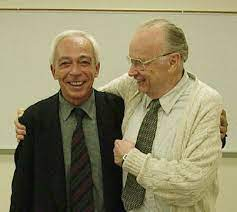
\includegraphics[width=1\textwidth]{Figures/BBB.jpeg} 
					\caption*{\tiny{F. Brezzi and I. Babu\v{s}ka}} 
				\end{figure} 
			\end{column} 
		\end{columns} 
	\end{frame}
	\begin{frame}{Boffi-Brezzi-Gastaldi observation}
		\begin{columns}[T] 
			\begin{column}{0.65\textwidth} 
			
			\vspace{0.2cm} 
			\begin{alertblock}{\textbf{Necessary and sufficient conditions}}
				When it comes to the eigenvalue problem, the inf-sup condition is \textbf{neither necessary nor sufficient}.
			\end{alertblock}
			\visible<2->{
				\begin{block}{\textbf{\color{oxfordblue}Q1-P0 Example}}
					Boffi, Brezzi and Gastaldi, showed that the \textbf{\color{oxfordblue} Q1-P0} finite element pair will lead to a converging eigenvalue problem, even if for this choice of element pair $\beta(h)\searrow 0$ as $h\to 0$.
				\end{block}
			}
			\end{column} 
			
			\begin{column}{0.35\textwidth} 
				\begin{figure} 
					\centering 
					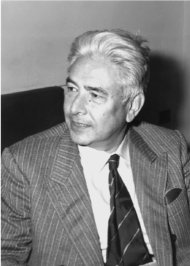
\includegraphics[width=0.8\textwidth]{Figures/DeGiorgi.jpg} 
					\caption*{\tiny{Enio De Giorgi, 1928--1996}} 
				\end{figure} 
			\end{column} 
		\end{columns} 
	\end{frame}
	\begin{frame}
		\frametitle{Boffi--Brezzi--Gastaldi conditions for Stokes}
		$\newline$
		\begin{itemize}
			\item<1->[\color{oxfordblue}$\blacktriangleright$] We say that $Q_h$ verifies the \textbf{\color{oxfordblue}weak approximability condition} if there exists $\gamma_1(h)$, such that for every $q \in \mathcal{L}^2_0(\Omega)$
				\begin{equation*}
					\underset{\vec{v}^h \in \mathbb{K}_h}{\sup} \frac{(\nabla\cdot\vec{v}^h,q)}{\norm{\vec{v}_h}_{H^1(\Omega)}} \leq \omega_1(h) \norm{q}_{\mathcal{L}^2(\Omega)} \; and \; \underset{h\to 0}{\lim}\,\gamma_1(h)=0.
				\end{equation*}
			\item<2->[\color{oxfordblue}$\blacktriangleright$] We say $V_h$ verifies the \textbf{\color{oxfordblue}strong approximability condition} if there exists $\gamma_2(h)$, such that for every $\vec{v} \in H^1_{0,0}(\Omega)\cap H^2(\Omega)$ 
				\begin{equation*}
					\underset{\vec{v}^h \in \mathbb{K}_h}{\inf} \norm{\vec{v}-\vec{v}^h}_{H^1(\Omega)} \leq \gamma_2(h)\norm{\vec{v}}_{H^2(\Omega)}\; and \; \underset{h\to 0}{\lim}\,\gamma_2(h)=0.
				\end{equation*}
		\end{itemize}
	\end{frame}
	\begin{frame}
		\frametitle{The divergence-free constraint}
		$\newline$
		$\newline$
		\begin{equation*}
			\boxed{
				b(\vec{v}^h,q^h)=(\nabla \cdot \vec{v}^h, q^h)_{\mathcal{L}^2(\Omega)}=0	
			}
		\end{equation*}
		$\newline$
		\visible<2->{
			Find $\vec{u}_h\!\in\!\mathbb{K}_{h}$ such that $\Forall \vec{v}_h\!\in\!\mathbb{K}_{h}$,
			\begin{equation*}
					\nu(\nabla \vec{u}^h,\nabla \vec{v}^h)_{\mathcal{L}^2(\Omega)}=\lambda_n^h \;(\vec{u}^h,\vec{v}^h)_{\mathcal{L}^2(\Omega)},
			\end{equation*}
			with $\lambda_n\in \mathbb{C}$, $\nu\in \mathbb{R}_{> 0}$ is the fluid viscosity and 
			\begin{equation*}
				\mathbb{K}_h=\Big\{\vec{v}^h\in V_h \;:\; b(\vec{v}^h,q^h) = 0, \Forall q^h\!\in\!Q_h\Big\}.
			\end{equation*}
		}
		\vspace{-0.3cm}
		\visible<3->{
			\begin{equation*}
				\boxed{\mathbb{K}_h\not\subset H^1_{0,0}(\Omega)}
			\end{equation*}
		}
	\end{frame}
	\begin{frame}
		\frametitle{Divergence-free discretisations}
		$\newline$
		\begin{equation*}
			\boxed{\nabla\cdot V_h\subset Q_h}
		\end{equation*}
		$\newline$
		\visible<2->{
			Under this hypothesis, we have the following result, i.e.
			\begin{equation*}
				b(\vec{v}^h,q^h)=(\nabla \cdot \vec{v}^h, q^h)_{\mathcal{L}^2(\Omega)}=0	\Leftrightarrow \nabla\cdot \vec{v}^h=0,
			\end{equation*}
			which implies the functions are point-wise \textbf{\color{oxfordblue}divergence-free}.
		}
		\visible<3->{
		\begin{equation*}
			\boxed{\mathbb{K}_h\subset H^1_{0,0}(\Omega)}
		\end{equation*}
		}
	\end{frame}
	\begin{frame}
		\frametitle{Divergence discretisations eigenvalue problem}
		$\newline$
		Find $\vec{u}_h\!\in\!\mathbb{K}_{h}$ such that $\Forall \vec{v}_h\!\in\mathbb{K}_{h}$,
		\begin{equation*}
				\nu(\nabla \vec{u}^h,\nabla \vec{v}^h)_{\mathcal{L}^2(\Omega)}=\lambda_n^h \;(\vec{u}^h,\vec{v}^h)_{\mathcal{L}^2(\Omega)},\label{eq:}
		\end{equation*}
		with $\nabla\cdot V_h\subset Q_h$, $\lambda_n\in \mathbb{C}$, $\nu\in \mathbb{R}_{> 0}$ is the fluid viscosity. 
		$\newline$
		\visible<2->{
			\begin{center}
				\color{oxfordblue} \textbf{This problem is well-posed and we can analyse it using Babu\v{s}ka-Osborn theory.}
			\end{center}
		}
	\end{frame}
	\begin{frame}
		\frametitle{Babu\v{s}ka--Osborn theory}
		\vspace{0.5cm}
		\begin{theorem}
			For each $n\in \mathbb{N}$, we have
			\begin{equation*}
				\lambda_n\leq \lambda_n^h \leq \lambda_n+C\underset{\vec{u}\in E,\;|\!|\vec{u}|\!|=1}{\sup}\;\underset{\vec{v}^h\in \mathbb{K}_{h}}{\inf}|\!| \vec{u}-\vec{v}_h |\!|_{H^{1}(\Omega)}^2
			\end{equation*}
			and there exists $\vec{w}^h_n\in \langle \vec{u}_{n}^h,\dots,\vec{u}_{n+m-1}^h\rangle$ such that
			\begin{equation*}
				|\!|\vec{u}_n-\vec{w}^h_n|\!|\leq C\underset{\vec{u}\in E,\;|\!|\vec{u}|\!|=1}{\sup}\;\underset{\vec{v}^h\in \mathbb{K}_{h}}{\inf}|\!| \vec{u}-\vec{v}_h |\!|_{H^{1}(\Omega)}
			\end{equation*}
			where $m$, $E$ and $\vec{u}_n$ are respectively the multiplicity, eigenspace and eigenvector corresponding to the eigenvalue $\lambda_n$.
		\end{theorem}
	\end{frame}
	\begin{frame}
		\frametitle{An example -- Type I mesh}
		\begin{lemma}
			Let $\vec{u} \in H^s(\Omega)\cap H^{1}_{0,0}(\Omega)$, with $s\geq 2$. On a special mesh obtained from a uniform square mesh dividing each cell along one of its diagonals there exists a $\vec{u}^h \in [\mathbb{P}^k(\mathcal{T}_h) ]^2$ such that
			\begin{align*}
				&\nabla\cdot \vec{u}_h = 0, \\
				&\norm{\vec{u}-\vec{u}_h}_{H^1(\Omega)} \leq C\abs{\vec{u}}_{H^s(\Omega)}\cdot \begin{cases}
					h^{\min(k-1,s-1)},\;\;\qquad k\in \{1,2,3\}\\
					h^{\min(k,s-1)}k^{(1-s)},\;\;\; k \geq 4
				\end{cases}
			\end{align*}
		\end{lemma}
	\end{frame}
	\begin{frame}
		\frametitle{An example -- Type I mesh}
		$\newline$
		\begin{equation*}
			\boxed{
				[\mathbb{P}^2(\mathcal{T}_h) ]^2 \; - \; \mathbb{P}^1_{disc}(\mathcal{T}_h) 
			}
		\end{equation*}
		\begin{figure}
			\centering
			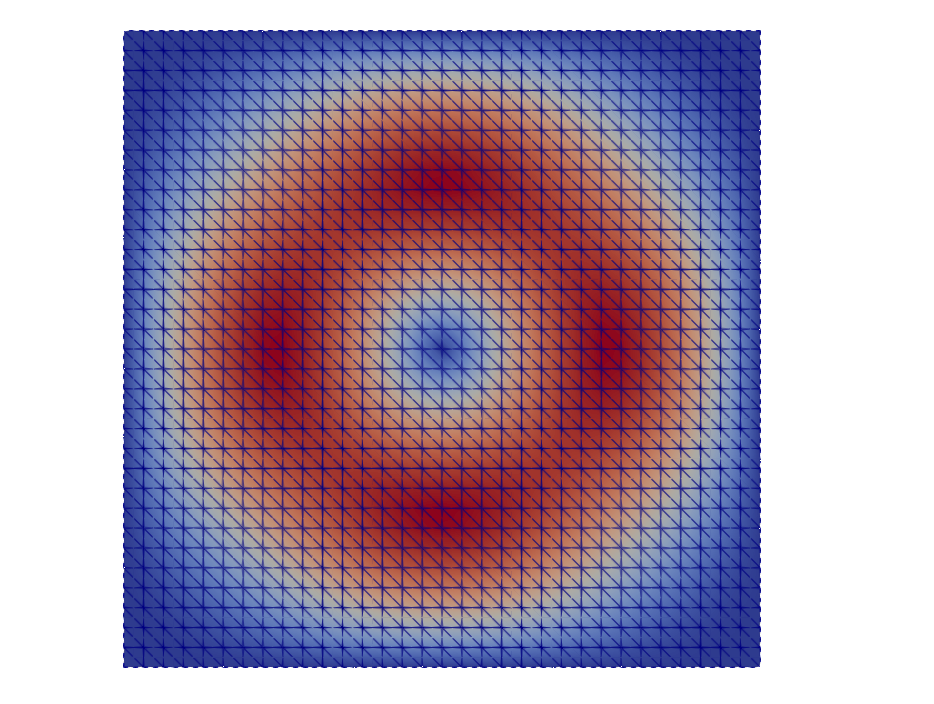
\includegraphics[scale=0.14]{Figures/P2P1DiscMesh.png}
			\qquad
			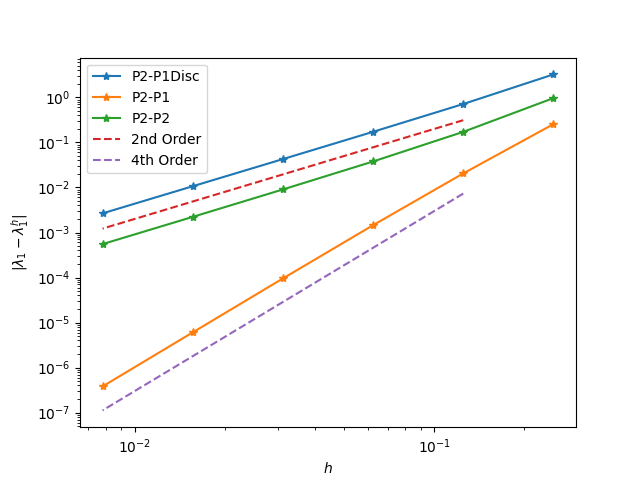
\includegraphics[scale=0.31]{Figures/P2P1Disc.png}
		\end{figure}
	\end{frame}
	\begin{frame}[fragile]
		\frametitle{Finite Element Exterior Calculus}
		\[
		\begin{tikzcd}
			0 \arrow{r} & H^2_0(\Omega) \arrow[d] \arrow{r}{\nabla\, \times} & \Big[H^1_0(\Omega)\Big]^2 \arrow[d] \arrow{r}{\nabla\,\cdot}& \mathcal{L}^2_0(\Omega)\arrow[d]  \arrow{r}& 0\\
			& \Sigma_h\arrow[d]  & \Phi_h \arrow{d}& \Xi_h \arrow{d}\\
			0 \arrow{r} & \Sigma_h \arrow{r}{\nabla\, \times} & \Phi_h \arrow{r}{\nabla\,\cdot}& \Xi_h^* \arrow{r}& 0
		\end{tikzcd}
		\]
	\end{frame}
	\begin{frame}
		\frametitle{Couple more example}	
		$\newline$
		\begin{itemize}
			\item [\color{oxfordblue}$\blacktriangleright$] $[\mathbb{P}^4(\mathcal{T}_h) ]^2 \; - \; \mathbb{P}^3_{disc}(\mathcal{T}_h)$, will be a converging scheme on a criss-cross mesh even if this choice of the element is not inf-sup stable.
			Best approximation estimates can be derived from the Morgan-Scott-Vogelius complex.
			\begin{figure}[h]
				\label{fig:DoF}
				$\newline$
				\centering
				\scalebox{0.45}{\tikzfig{Figures/DoF}}
			\end{figure}
		\end{itemize}
	\end{frame} 
	\begin{frame}
		\frametitle{Couple more example}	
		$\newline$
		\begin{itemize}
			\item [\color{oxfordblue}$\blacktriangleright$] $[\mathbb{P}^2(\mathcal{T}_h) ]^2 \; - \; \mathbb{P}^2(\mathcal{T}_h)$, will be a converging scheme on a barycentrically refined mesh even if this choice of the element is not inf-sup stable.
			Best approximation estimates can be derived from Hsieh-Clough-Tocher complex.
			\begin{figure}[h]
				\label{fig:DoF}
				$\newline$
				\centering
				\scalebox{0.45}{\tikzfig{Figures/DoF3}}
			\end{figure}
		\end{itemize}
	\end{frame} 
	\begin{frame}
		\frametitle{Conclusions}
		$\newline$
		$\newline$
		\begin{minipage}{5cm}
			\begin{itemize}
				\item<1->[\color{oxfordblue}$\blacktriangleright$] There is no need to characterise the range of the divergence operator! \textbf{\color{oxfordblue} This is crucial for three-dimensional problems.}
				\item<2->[\color{oxfordblue}$\blacktriangleright$] A wide variety of finite element space pairs can be used even if they are not \textbf{\color{oxfordblue} inf-sup} stable.
			\end{itemize}
		\end{minipage}
		\begin{minipage}{5cm}
			\begin{figure}
				\centering
				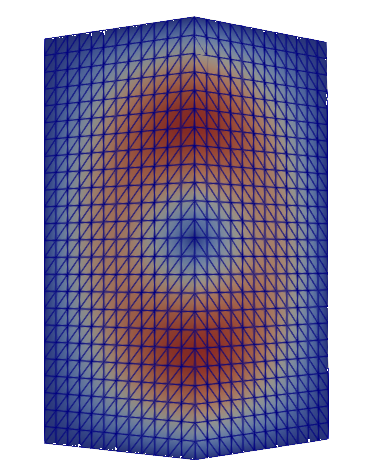
\includegraphics[scale=0.23]{Figures/3D.png}
			\end{figure}
		\end{minipage}
		$\newline$
		\visible<3->{
			\begin{center}
				\textbf{\color{oxfordblue} Thank you for your attention !}
			\end{center}
		}
	\end{frame}
\end{document}
